\documentclass{article}
\usepackage[margin=1in]{geometry}
\usepackage{float}
\usepackage{graphicx}
\usepackage{float}
\usepackage{xcolor}
\usepackage{listings}
\usepackage{tcolorbox}

% --- Color Definitions ---
\definecolor{terminalbg}{RGB}{30, 30, 30}     % Dark gray/black for terminal
\definecolor{terminaltext}{RGB}{212, 212, 212} % Light gray for text
\definecolor{quotebg}{RGB}{245, 247, 250}      % Very light blue/gray for quote
\definecolor{quoteline}{RGB}{41, 128, 185}     % Blue accent line for quote

% --- Code Block (Listings) Setup ---
\lstdefinestyle{darkterminal}{
    backgroundcolor=\color{terminalbg},
    basicstyle=\ttfamily\color{terminaltext}\small,
    breaklines=true,
    frame=single,
    rulecolor=\color{terminalbg}, % Hides the frame border by making it match the bg
    framesep=8pt,                 % Padding inside the box
    xleftmargin=8pt,
    xrightmargin=8pt,
    showstringspaces=false
}
\lstset{style=darkterminal}

% --- Quote Box (tcolorbox) Setup ---
\newtcolorbox{fancyquote}{
    colback=quotebg,
    colframe=quoteline,
    boxrule=0pt,       % No border on top/right/bottom
    leftrule=4pt,      % Thick accent line on the left
    arc=4pt,           % Slightly rounded corners
    boxsep=5pt,
    left=10pt,
    right=10pt,
    fontupper=\itshape % Makes the quote text italic
}
\lstset{breaklines=true}

\title{IoT - Challenge 2}
\author{Raul Agolli - Team Leader \\\\ Gabriele Lorenzo Singe}
\date{April 2026}

\begin{document}

\maketitle


\section{CQ1}

\begin{fancyquote}
    \textbf{CQ1a)} Find all NON Confirmable DELETE requests directed to the coap.me server that received a successful response. Take note of the MID of such requests.\\
    \textbf{CQ1b)} How many of the requests found in point CQ1a) actually obtained the desired outcome?
\end{fancyquote}

\vspace{0.3cm}

\noindent
\begin{minipage}{\linewidth}
\subsection{Find \textit{"coap.me"} IP address}
This can be done by looking up DNS requests:
\begin{lstlisting}
dns.qry.name == "coap.me" && dns.flags.response == 1
\end{lstlisting}
\vspace{-0.2cm}
\begin{figure}[H]
    \centering
    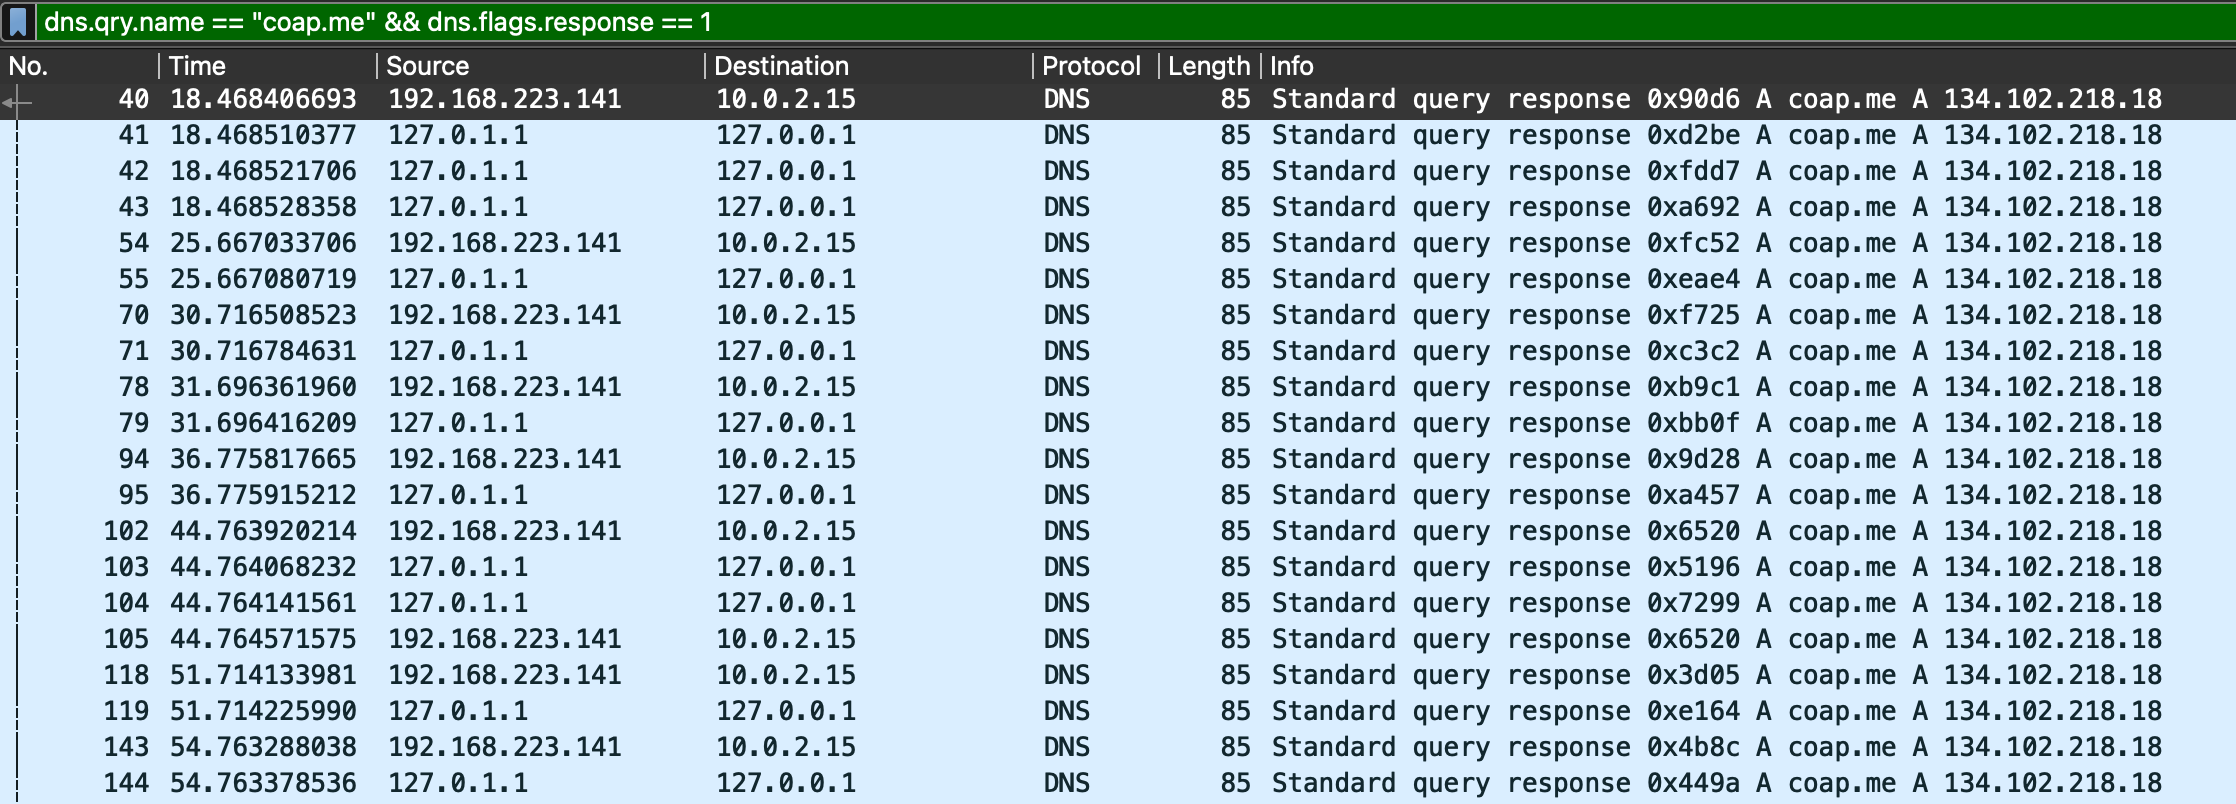
\includegraphics[width=0.9\linewidth]{images/coap_ip_wireshark.png}
\end{figure}
From these \textbf{DNS requests}, it is possible to retrieve the \textbf{coap.me} IP address: \textbf{134.102.218.18}.
\end{minipage}

\vspace{0.5cm}

\subsection{CQ1a - Find all NON Confirmable DELETE requests directed to the coap.me server that received a successful response. Take note of the MID of such requests}

Now 2 filters have to be used to identify if the request received a "successful response".

\begin{figure}[H]
    \centering
    \begin{minipage}[t]{0.48\textwidth}
        \textbf{Filter 1: Isolate NON DELETE Requests}
\begin{lstlisting}
ip.dst == 134.102.218.18 && coap.type == 1 && coap.code == 4
\end{lstlisting}
\begin{lstlisting}
tshark -r A.pcapng -Y "ip.dst == 134.102.218.18 && coap.type == 1 && coap.code == 4" -T fields -e coap.token -e coap.mid -e coap.opt.uri_path > non_deletes.txt
\end{lstlisting}

        First, we extract the Token, MID, and Uri-Path of all NON (type == 1) DELETE (code == 4) requests directed to the server.
        \vspace{0.2cm}
    \end{minipage}\hfill
    \begin{minipage}[t]{0.48\textwidth}
        \textbf{Filter 2: Isolate "2.02 Deleted" Responses}
\begin{lstlisting}
ip.src == 134.102.218.18 && coap.code == 66
\end{lstlisting}
\begin{lstlisting}
tshark -r A.pcapng -Y "ip.src == 134.102.218.18 && coap.code == 66" -T fields -e coap.token > 202_responses.txt
\end{lstlisting}
        We filter the traffic coming from the server for the specific 2.02 Deleted response (code == 66) and extract their Tokens.
        \vspace{0.2cm}
    \end{minipage}
\end{figure}

\noindent
\begin{minipage}{\linewidth}
The outputs of the two commands are saved in two files. To respond to question \textbf{CQ1a}, the two outputs are compared:

\begin{figure}[H]
    \centering
    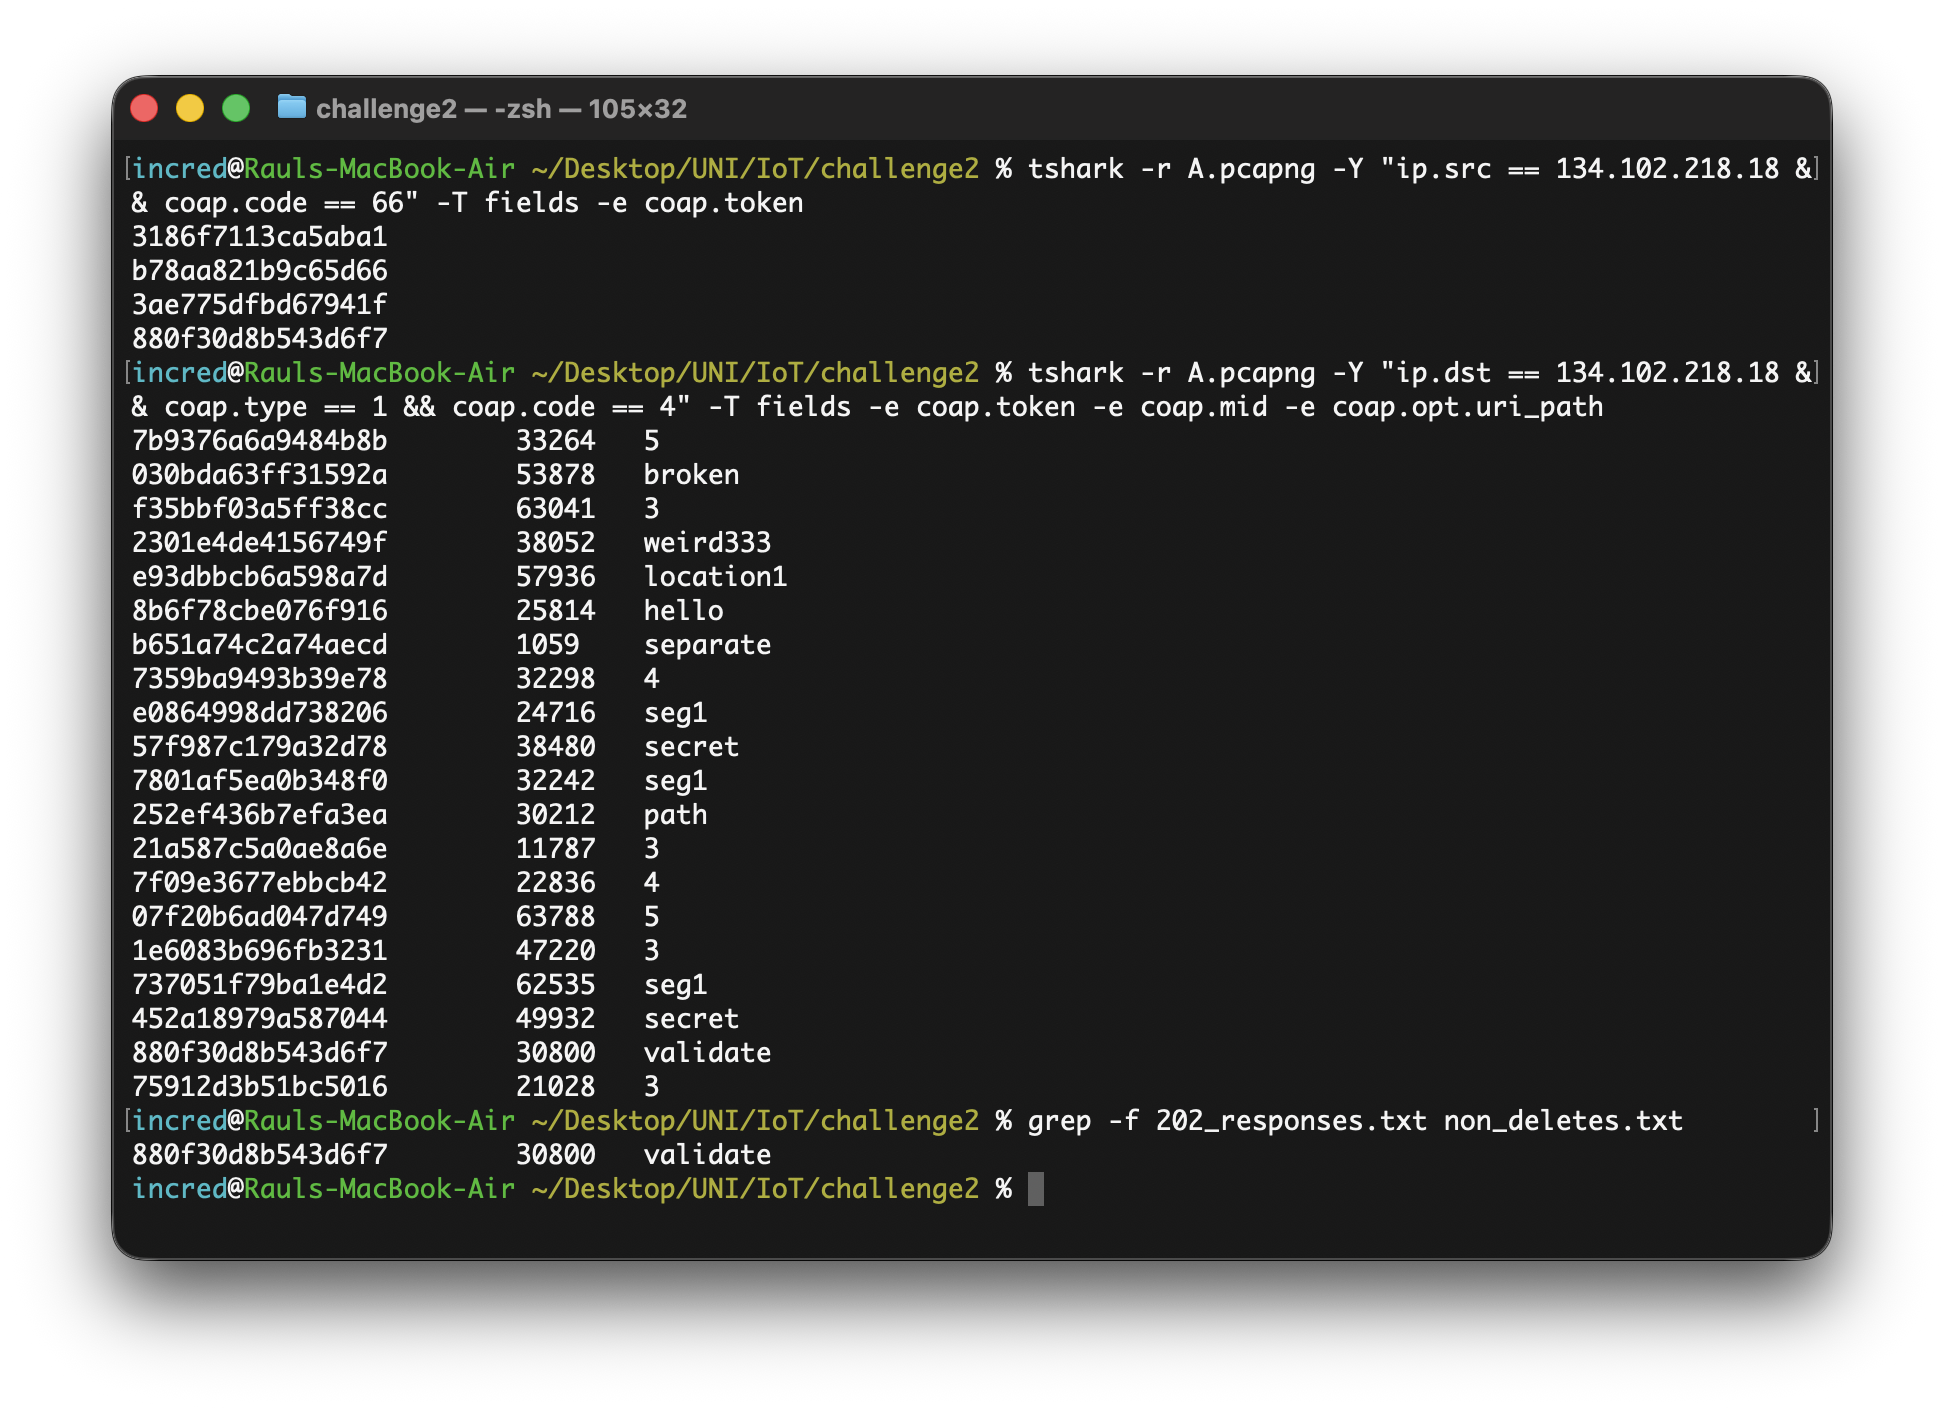
\includegraphics[width=0.65\linewidth]{images/cq1-result.png}
\end{figure}

By cross-referencing the Tokens from the successful responses against our initial list of requests, we isolate the DELETE requests that the server actively accepted.
\end{minipage}

\vspace{0.5cm}

\textbf{\huge Answer CQ1a: 30800}

\vspace{0.5cm}

\noindent
\begin{minipage}{\linewidth}
\subsection{CQ1b - How many of the requests found in point CQ1a) actually obtained the desired outcome?}
Receiving a \texttt{2.02 Deleted} response only confirms that the server \textit{accepted} the request. In IoT environments, this does not guarantee the resource was physically removed. To prove the desired outcome was achieved, it is necessary to observe the network traffic for a subsequent \texttt{GET} request directed to the exact same \texttt{Uri-Path}. If the deletion was truly successful, the server must respond to that new \texttt{GET} request with a \texttt{4.04 Not Found} (Code 132) error.

\subsubsection*{Extract the Deleted URIs}
Extract the \texttt{Uri-Path} (3rd column) from the successfully accepted DELETEs found in CQ1a.
\begin{lstlisting}[language=bash]
awk '{print $3}' accepted_deletes.txt > deleted_uris.txt
\end{lstlisting}
\end{minipage}

\vspace{0.3cm}

\noindent
\begin{minipage}{\linewidth}
\subsubsection*{Isolate All GET Requests}
Extract the Token and \texttt{Uri-Path} for all \texttt{GET} requests (\texttt{code == 1}) sent to the server.
\begin{lstlisting}[language=bash]
tshark -r A.pcapng -Y "ip.dst == 134.102.218.18 && coap.code == 1" -T fields -e coap.token -e coap.opt.uri_path > all_gets.txt
\end{lstlisting}
\end{minipage}

\vspace{0.3cm}

\noindent
\begin{minipage}{\linewidth}
\subsubsection*{Find GET Requests Targeting the Deleted URIs}
Cross-reference the list of deleted URIs against all GET requests to find attempts to access the deleted resources. The \texttt{-w} and \texttt{-F} flags force exact string matching to prevent false positives from hexadecimal substring overlaps.
\begin{lstlisting}[language=bash]
grep -w -F -f deleted_uris.txt all_gets.txt | awk '{print $1}' > get_tokens.txt
\end{lstlisting}


\vspace{0.3cm}

\noindent

\subsubsection*{Isolate "4.04 Not Found" Responses}
Extract the Tokens of all \texttt{4.04 Not Found} (\texttt{code == 132}) responses originating from the server.
\begin{lstlisting}[language=bash]
tshark -r A.pcapng -Y "ip.src == 134.102.218.18 && coap.code == 132" -T fields -e coap.token > 404_responses.txt
\end{lstlisting}


\vspace{0.3cm}

\noindent
\subsubsection*{Correlate to Prove Deletion}
Compare the Tokens of the \texttt{4.04} responses against the Tokens of the \texttt{GET} requests that targeted the deleted URIs. Piping the output to \texttt{wc -l} counts the exact number of verified deletions.
\begin{lstlisting}[language=bash]
grep -w -F -f 404_responses.txt get_tokens.txt | wc -l
\end{lstlisting}

\vspace{0.3cm}

\begin{figure}[H]
    \centering
    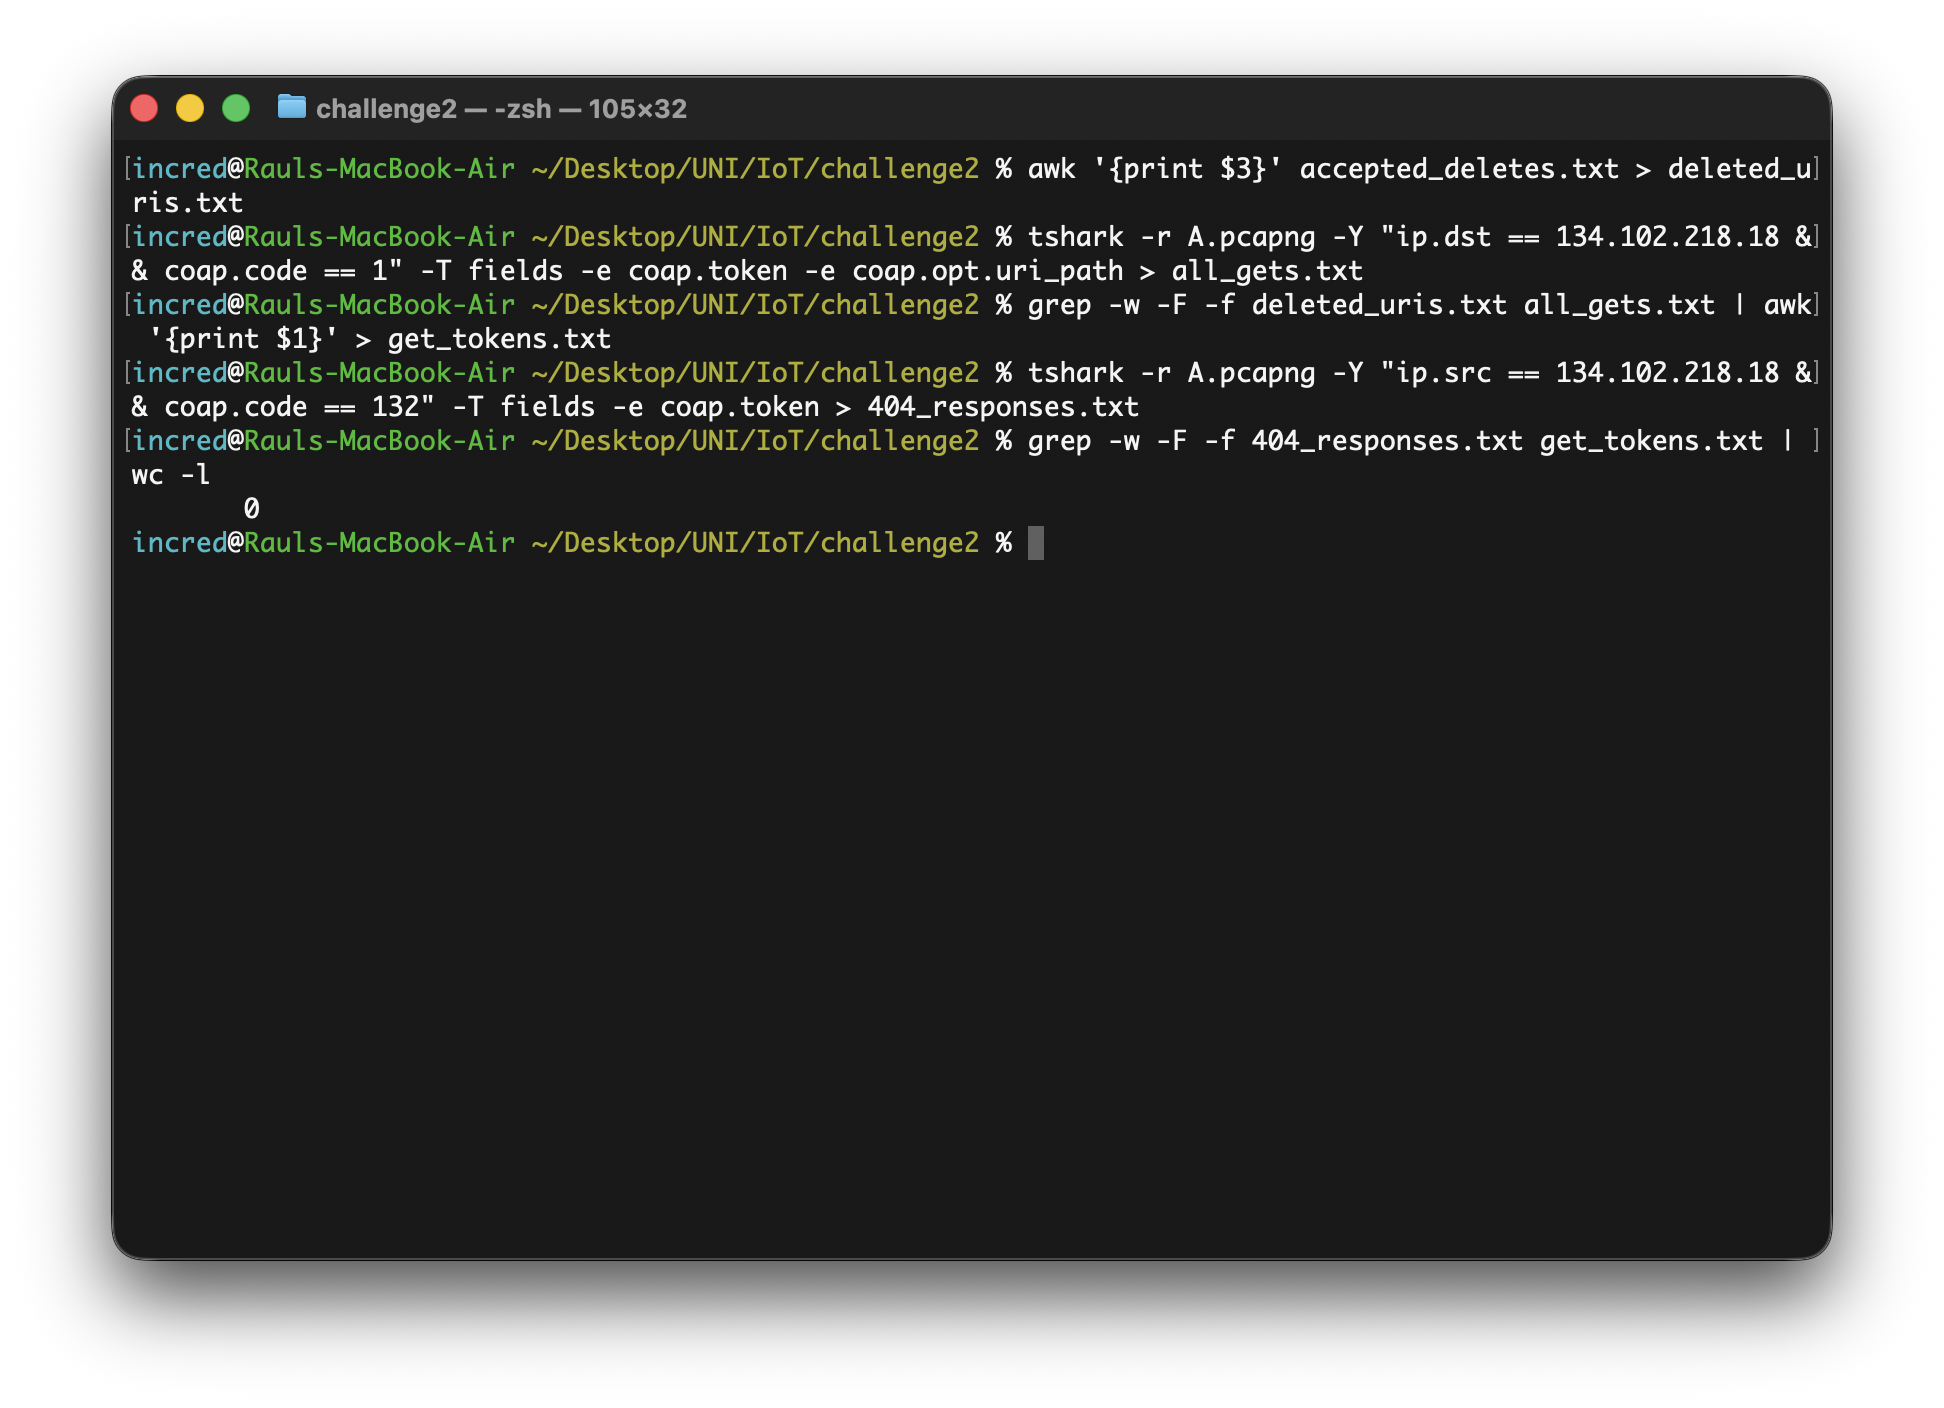
\includegraphics[width=0.7\linewidth]{images/cq1b-result.png}
\end{figure}

\textbf{\huge Answer CQ1b: 0}

\vspace{0.3cm}
\textit{Conclusion: The result of 0 proves that while the coap.me server politely accepted the DELETE commands (replying with 2.02), it did not actually delete the resources, as subsequent queries for those paths did not return a 4.04 Not Found.}
\end{minipage}


\section{CQ2}

\begin{fancyquote}
    \textbf{Question:}\\
    How many CoAP resources in the local server received the same number of unique unsuccessful Confirmable POST and PUT requests?\\
    Assuming a resource receives $X$ different CON unsuccessful POST requests and $Y$ different CON unsuccessful PUT requests, how many resources have $X=Y$, with $X>0$?
    
    \vspace{0.1cm}
    \textit{!! Consider unsuccessful only if there is a response stating it is not successful !!}
\end{fancyquote}

\vspace{0.3cm}

\noindent
\begin{minipage}{\linewidth}
\subsection*{Isolate Unsuccessful Responses}
An "unsuccessful" response in CoAP means the server returned a Client Error (\texttt{4.xx}) or a Server Error (\texttt{5.xx}). Any response code between 128 and 191 is an explicit unsuccessful response.

\textbf{Filter:}
\begin{lstlisting}
ip.src == 127.0.0.1 && coap.code >= 128 && coap.code <= 191
\end{lstlisting}
This extracts just the tokens of all explicit error responses sent by the server and saves them to a text file.

\begin{figure}[H]
    \centering
    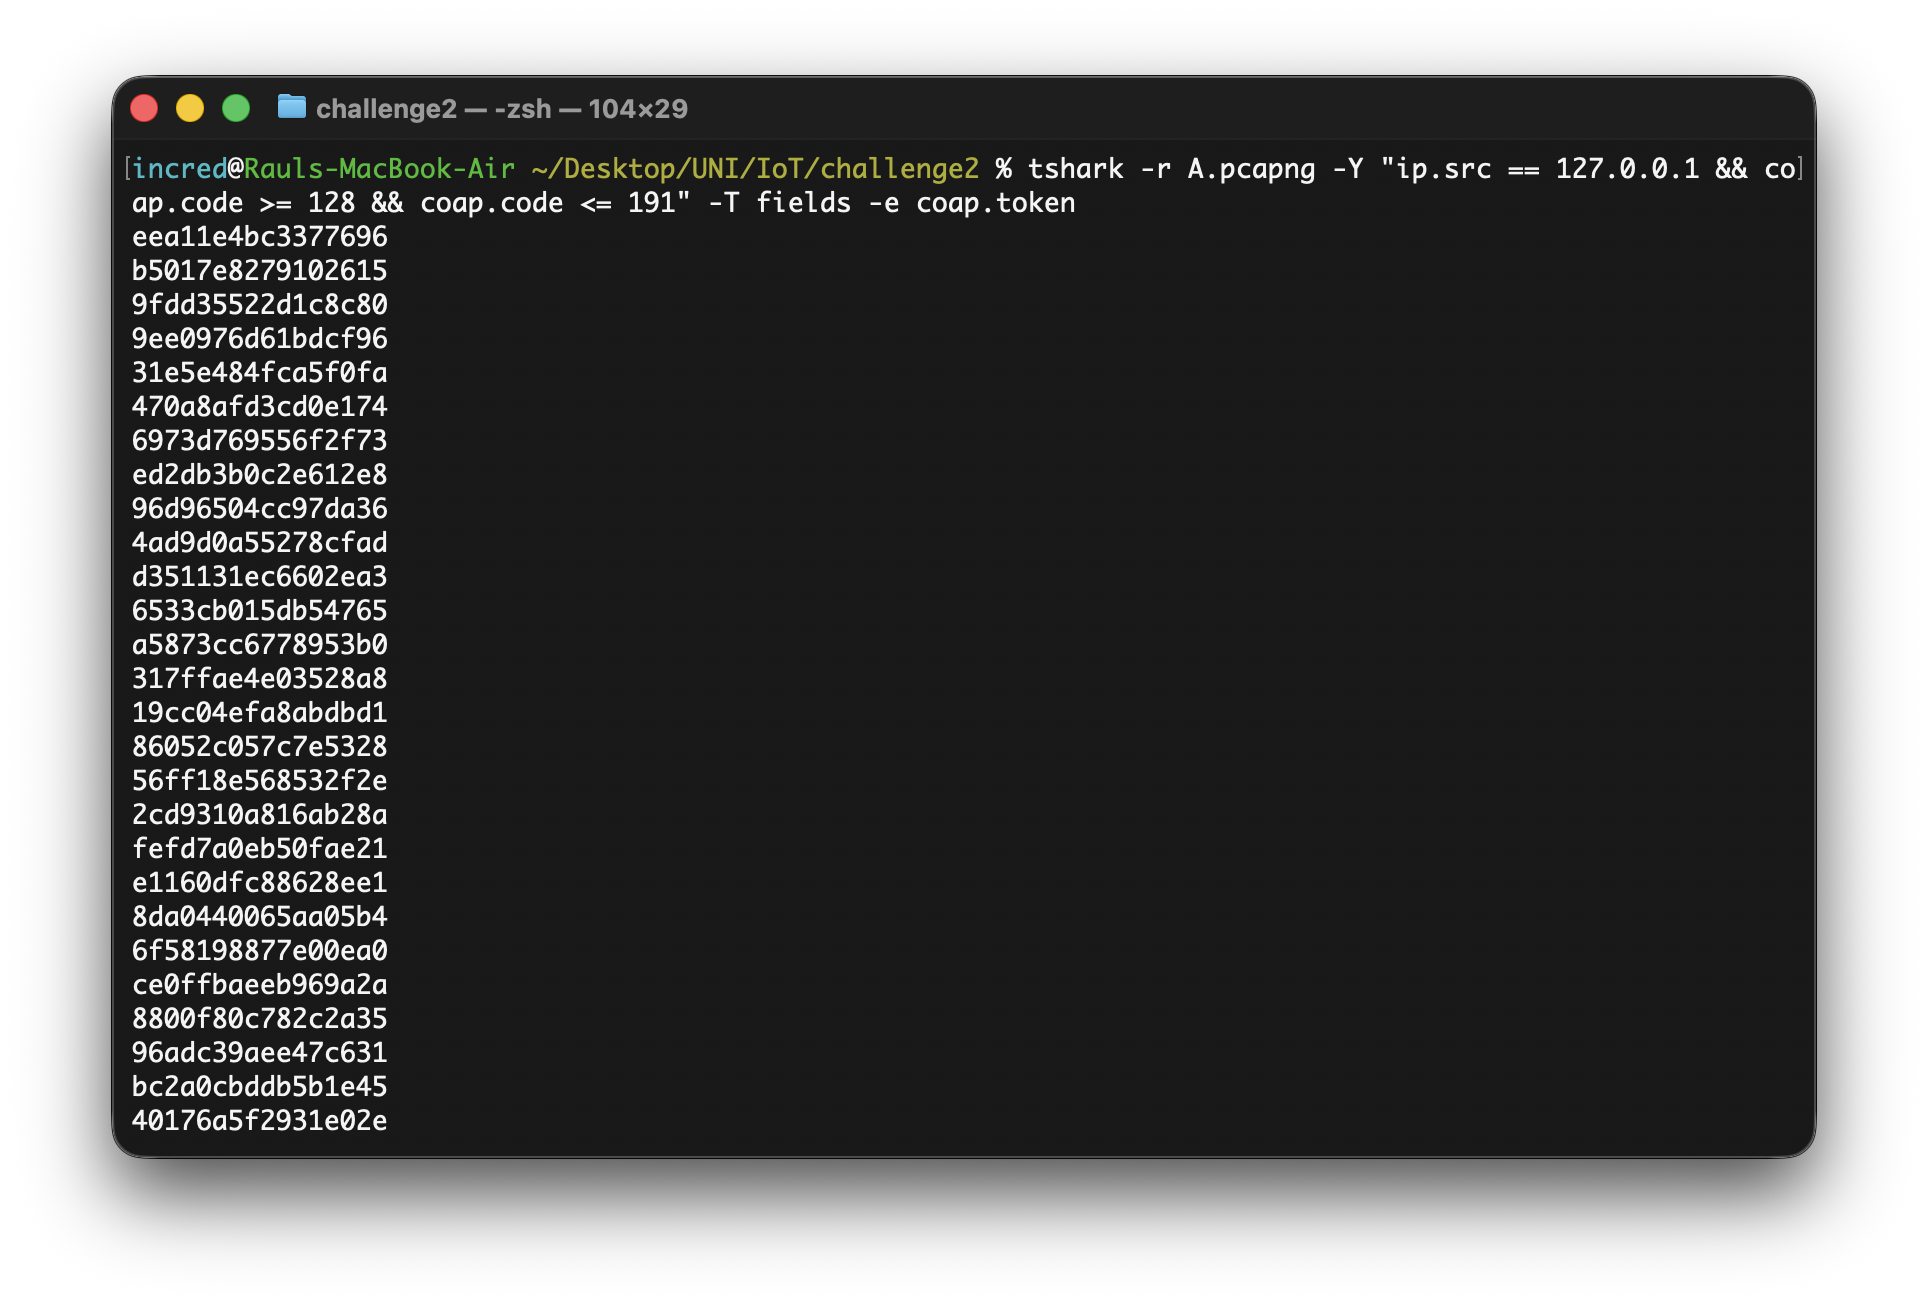
\includegraphics[width=0.75\linewidth]{images/cq2-unsuccessful.png}
\end{figure}
Output is saved in \textbf{\texttt{unsuccessful\_tokens.txt}}
\end{minipage}

\vspace{0.5cm}

\subsection*{Extract CON POST and CON PUT Requests}
We need to capture all Confirmable (\texttt{coap.type == 0}) POST (\texttt{coap.code == 2}) and PUT (\texttt{coap.code == 3}) requests directed at the server. We must extract both the Token (to match with the errors) and the URI Path (which represents the resource).

\begin{figure}[H]
    \centering
    \begin{minipage}[t]{0.48\textwidth}
        \textbf{Extract CON POST requests:}
\begin{lstlisting}
ip.dst == 127.0.0.1 && 
coap.type == 0 && coap.code == 2
\end{lstlisting}
        \vspace{0.1cm}
        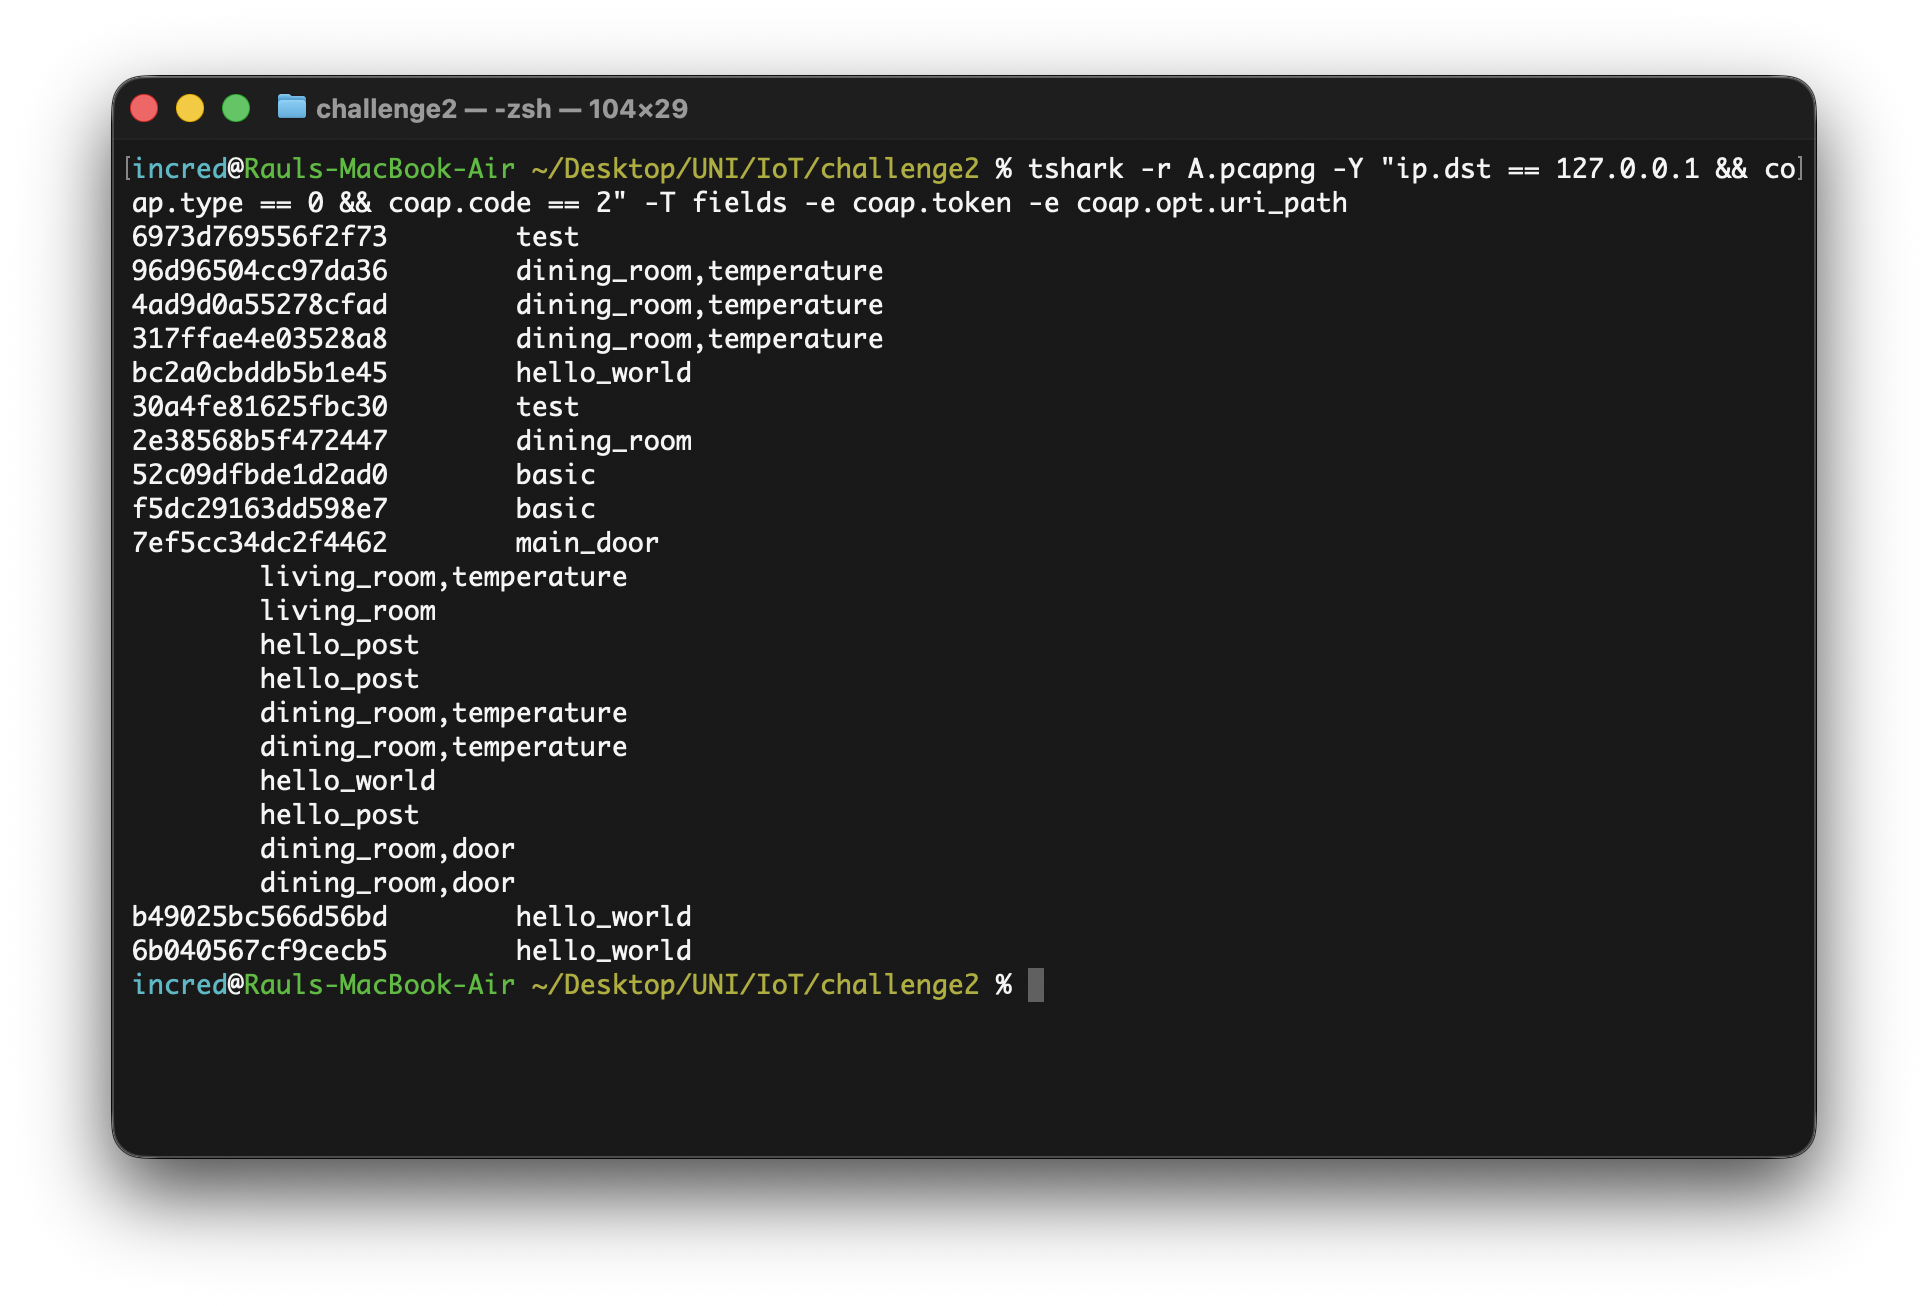
\includegraphics[width=\linewidth]{images/cq2-post.png}
        \vspace{0.1cm}\\
        Output saved in \textbf{\texttt{all\_post\_reqs.txt}}
    \end{minipage}\hfill
    \begin{minipage}[t]{0.48\textwidth}
        \textbf{Extract CON PUT requests:}
\begin{lstlisting}
ip.dst == 127.0.0.1 && 
coap.type == 0 && coap.code == 3
\end{lstlisting}
        \vspace{0.1cm}
        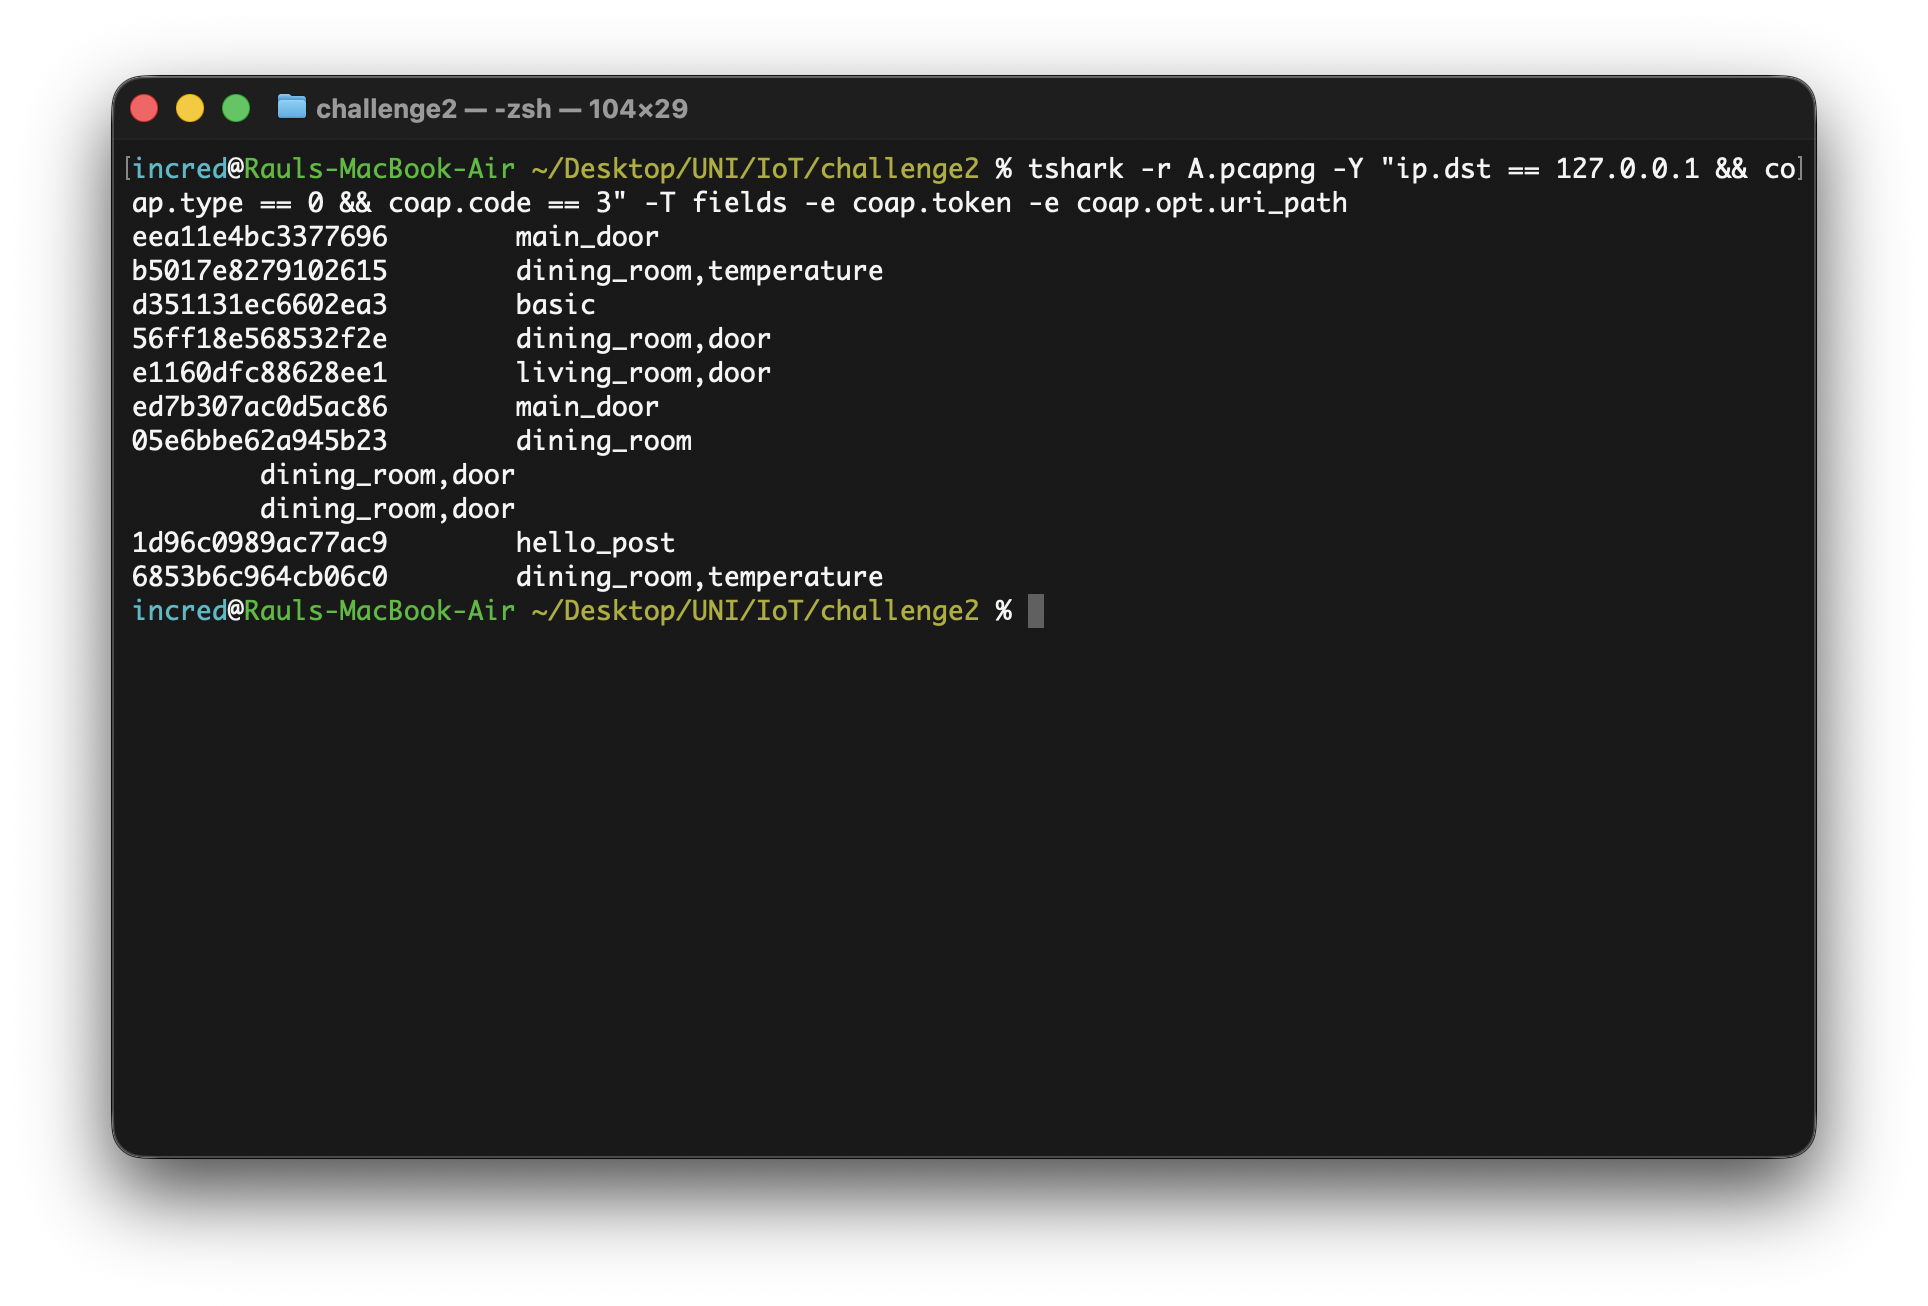
\includegraphics[width=\linewidth]{images/cq2-put.png}
        \vspace{0.1cm}\\
        Output saved in \textbf{\texttt{all\_put\_reqs.txt}}
    \end{minipage}
\end{figure}

\vspace{0.5cm}

\subsection*{Filter, Remove Duplicates and Count}
Identify which requests failed, count only unique requests, then add them by resource.

\begin{figure}[H]
    \centering
    \begin{minipage}[t]{0.48\textwidth}
        \subsubsection*{Find X (POST requests)}
\begin{lstlisting}
grep -f unsuccessful_tokens.txt all_post_reqs.txt | sort -u | awk '{print $2}' | sort | uniq -c | awk '{print $2, $1}' | sort > post_counts.txt
\end{lstlisting}
        \vspace{0.1cm}
        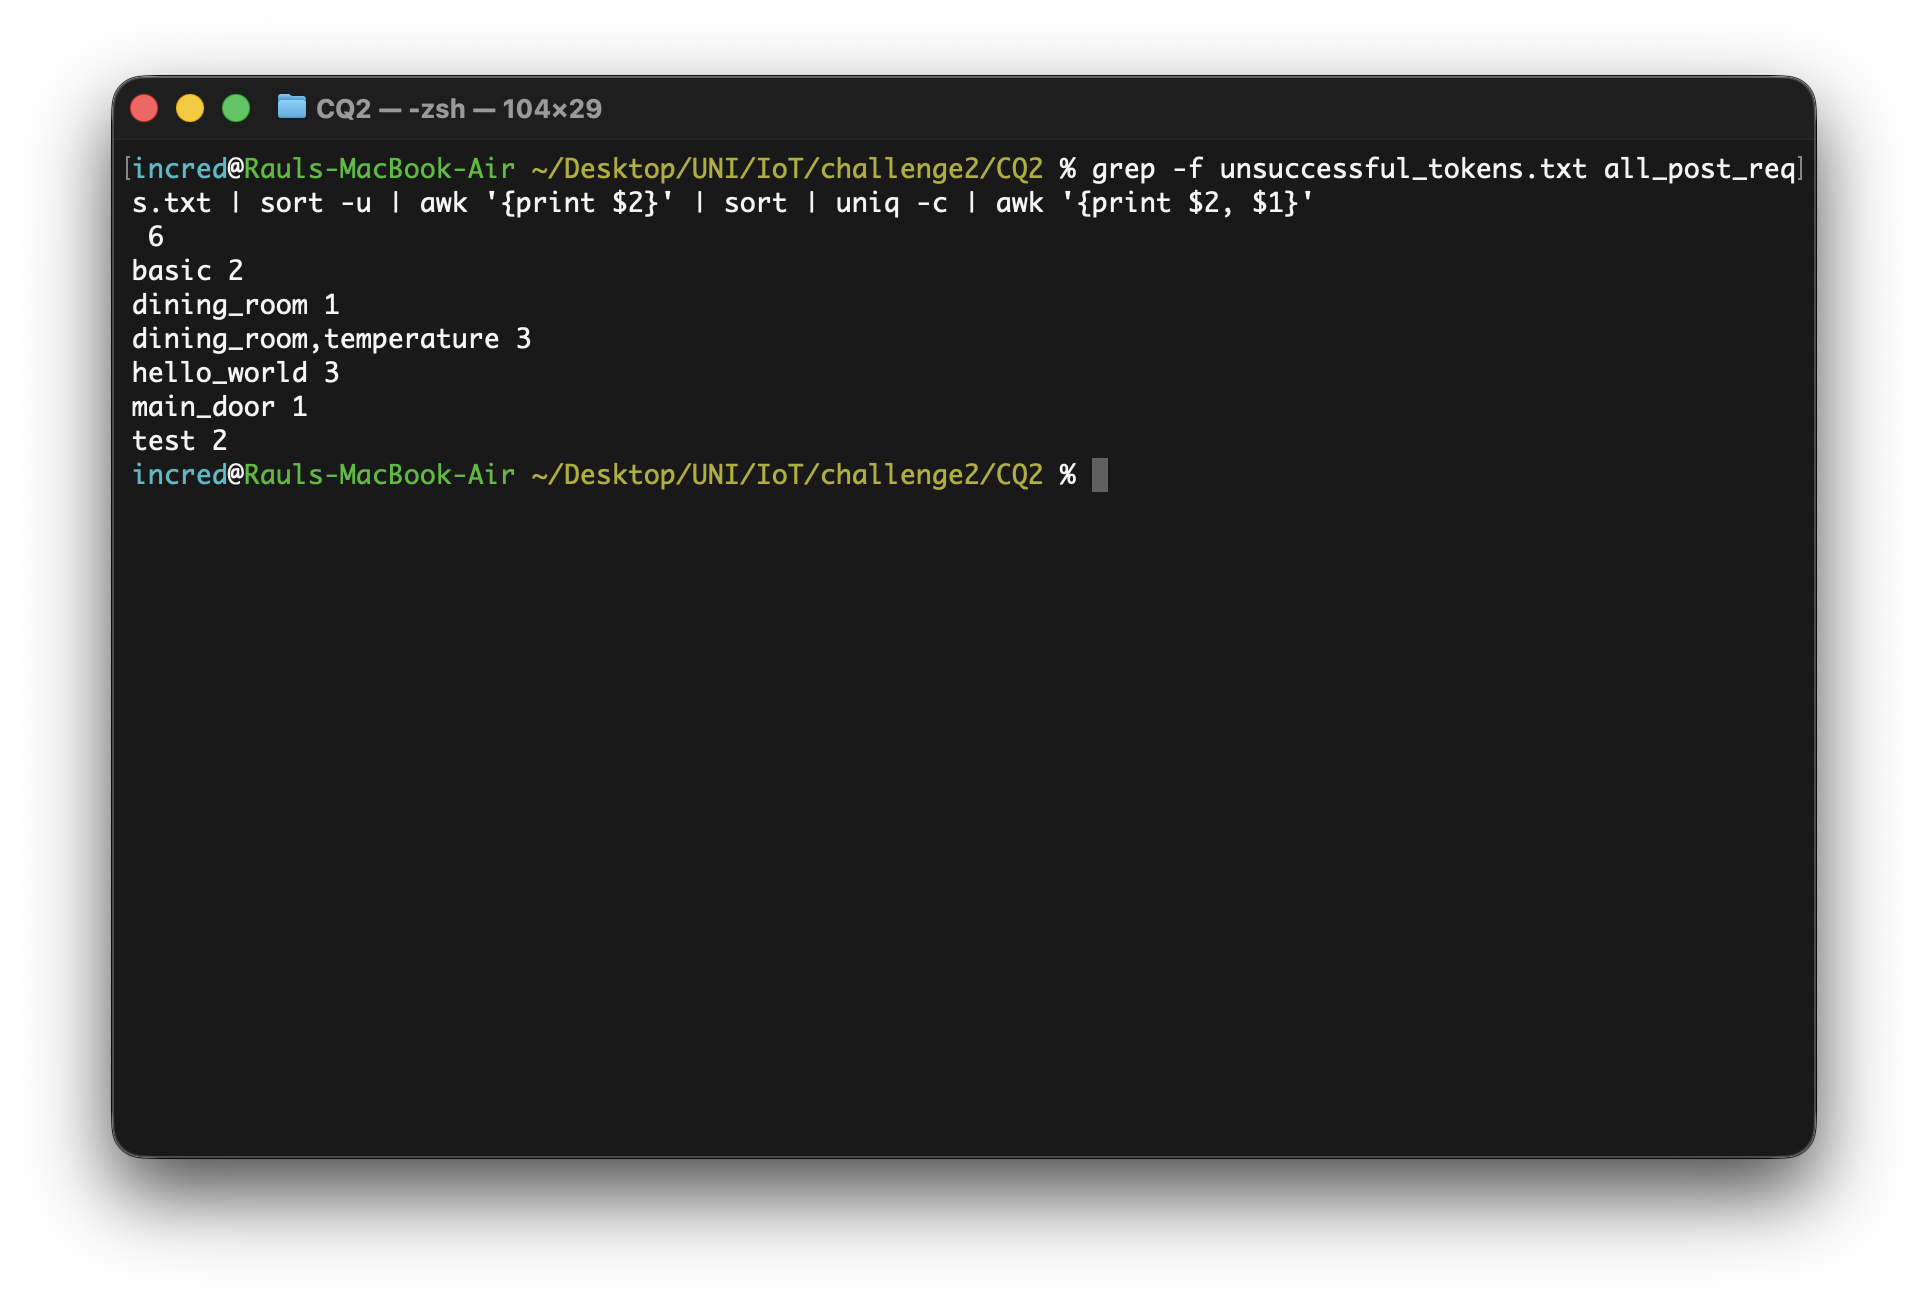
\includegraphics[width=\linewidth]{images/cq2-x.png}
        \vspace{0.1cm}\\
        Output saved in \textbf{\texttt{post\_counts.txt}}
    \end{minipage}\hfill
    \begin{minipage}[t]{0.48\textwidth}
        \subsubsection*{Find Y (PUT requests)}
\begin{lstlisting}
grep -f unsuccessful_tokens.txt all_put_reqs.txt | sort -u | awk '{print $2}' | sort | uniq -c | awk '{print $2, $1}' | sort > put_counts.txt
\end{lstlisting}
        \vspace{0.1cm}
        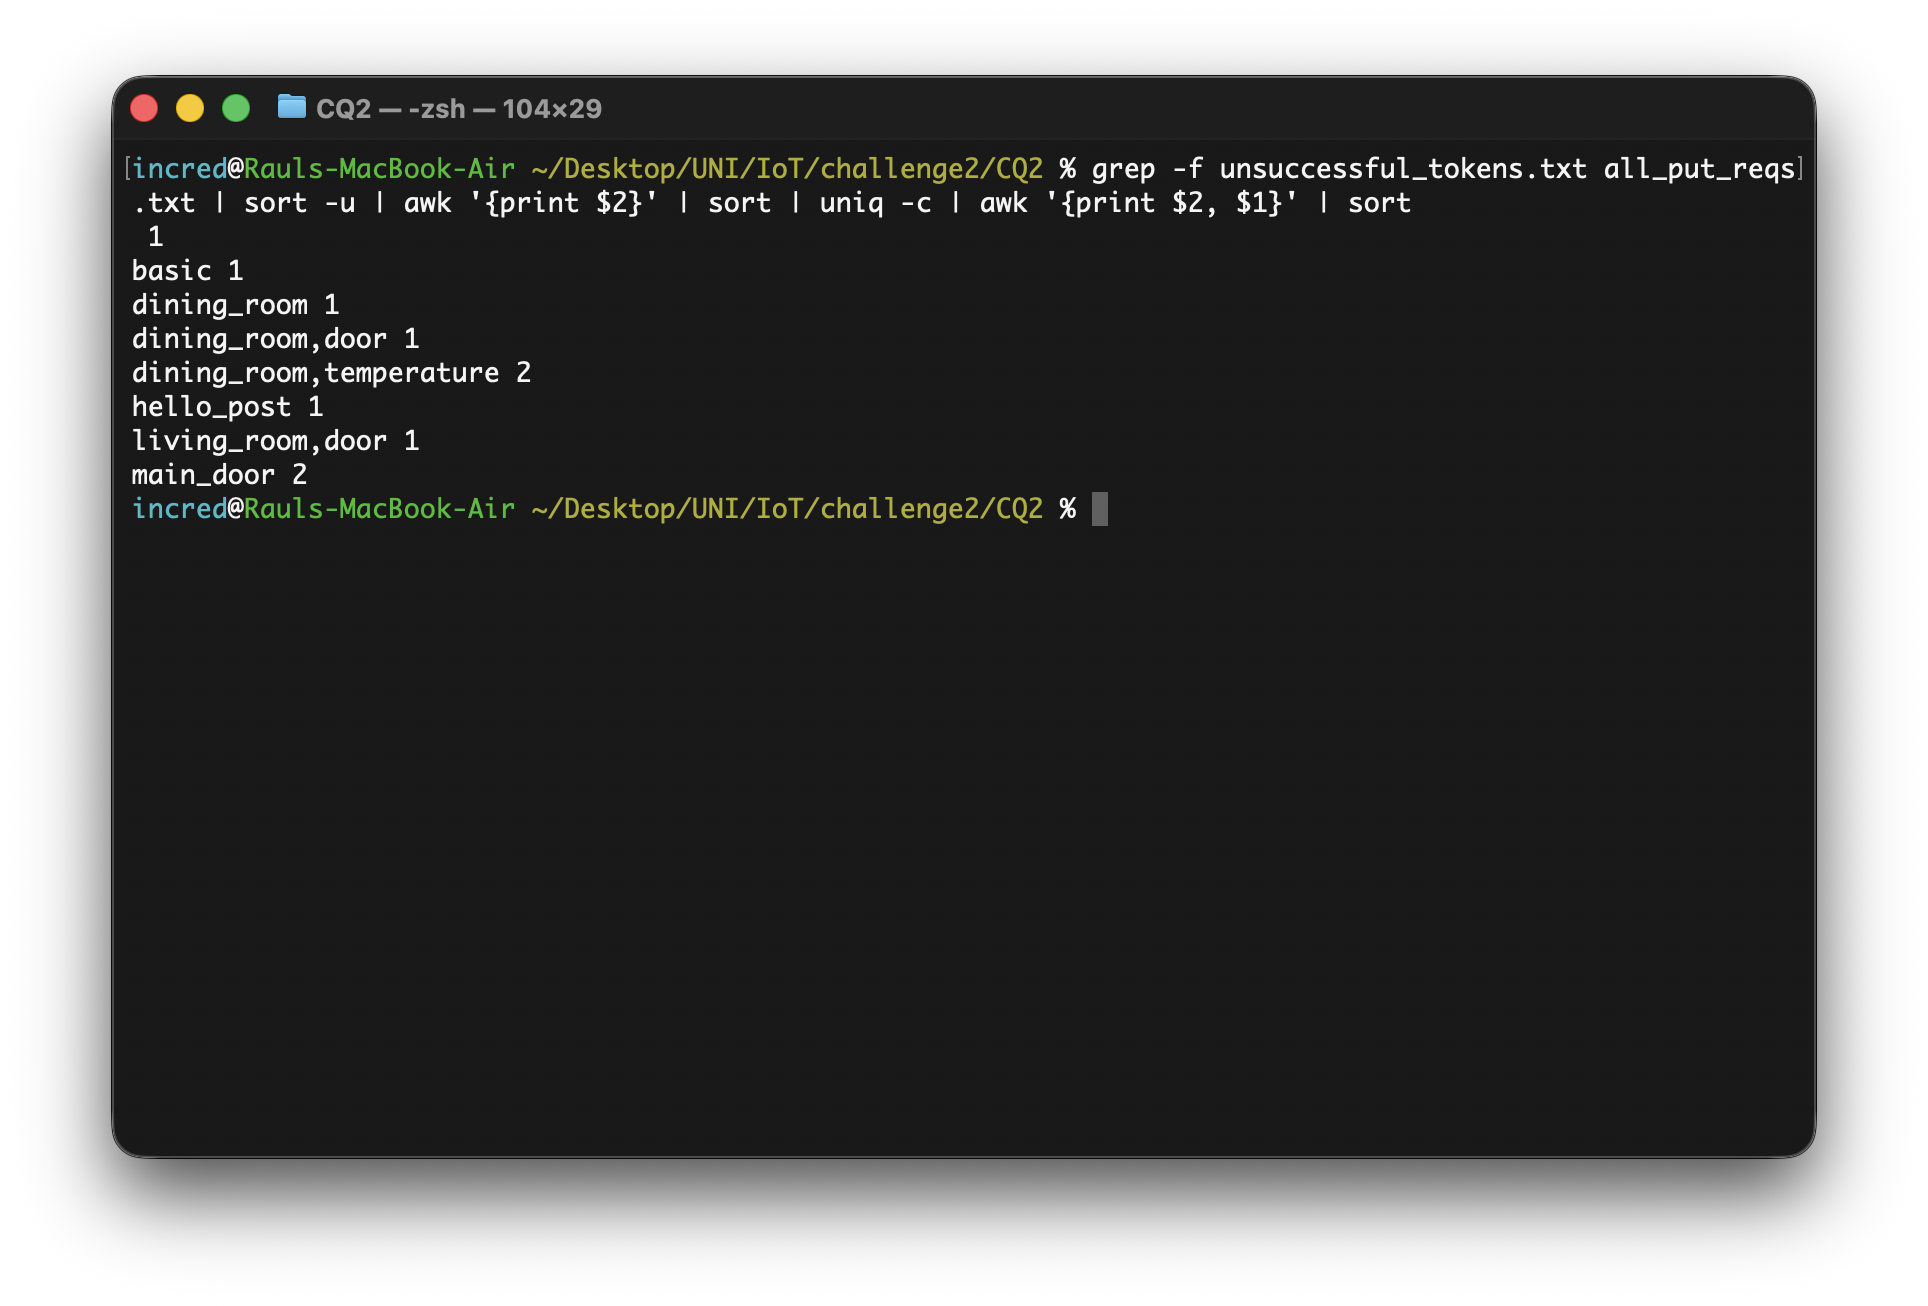
\includegraphics[width=\linewidth]{images/cq2-y.png}
        \vspace{0.1cm}\\
        Output saved in \textbf{\texttt{put\_counts.txt}}
    \end{minipage}
\end{figure}

\vspace{0.5cm}

\noindent
\begin{minipage}{\linewidth}
\subsection*{Compare the Results (Where $X = Y, X > 0$)}
Join the previous files together based on the resource name, check if the counts match, and verify that the count is greater than zero.
\begin{lstlisting}
join post_counts.txt put_counts.txt | awk '$2 == $3 && $2 > 0'
\end{lstlisting}

\begin{figure}[H]
    \centering
    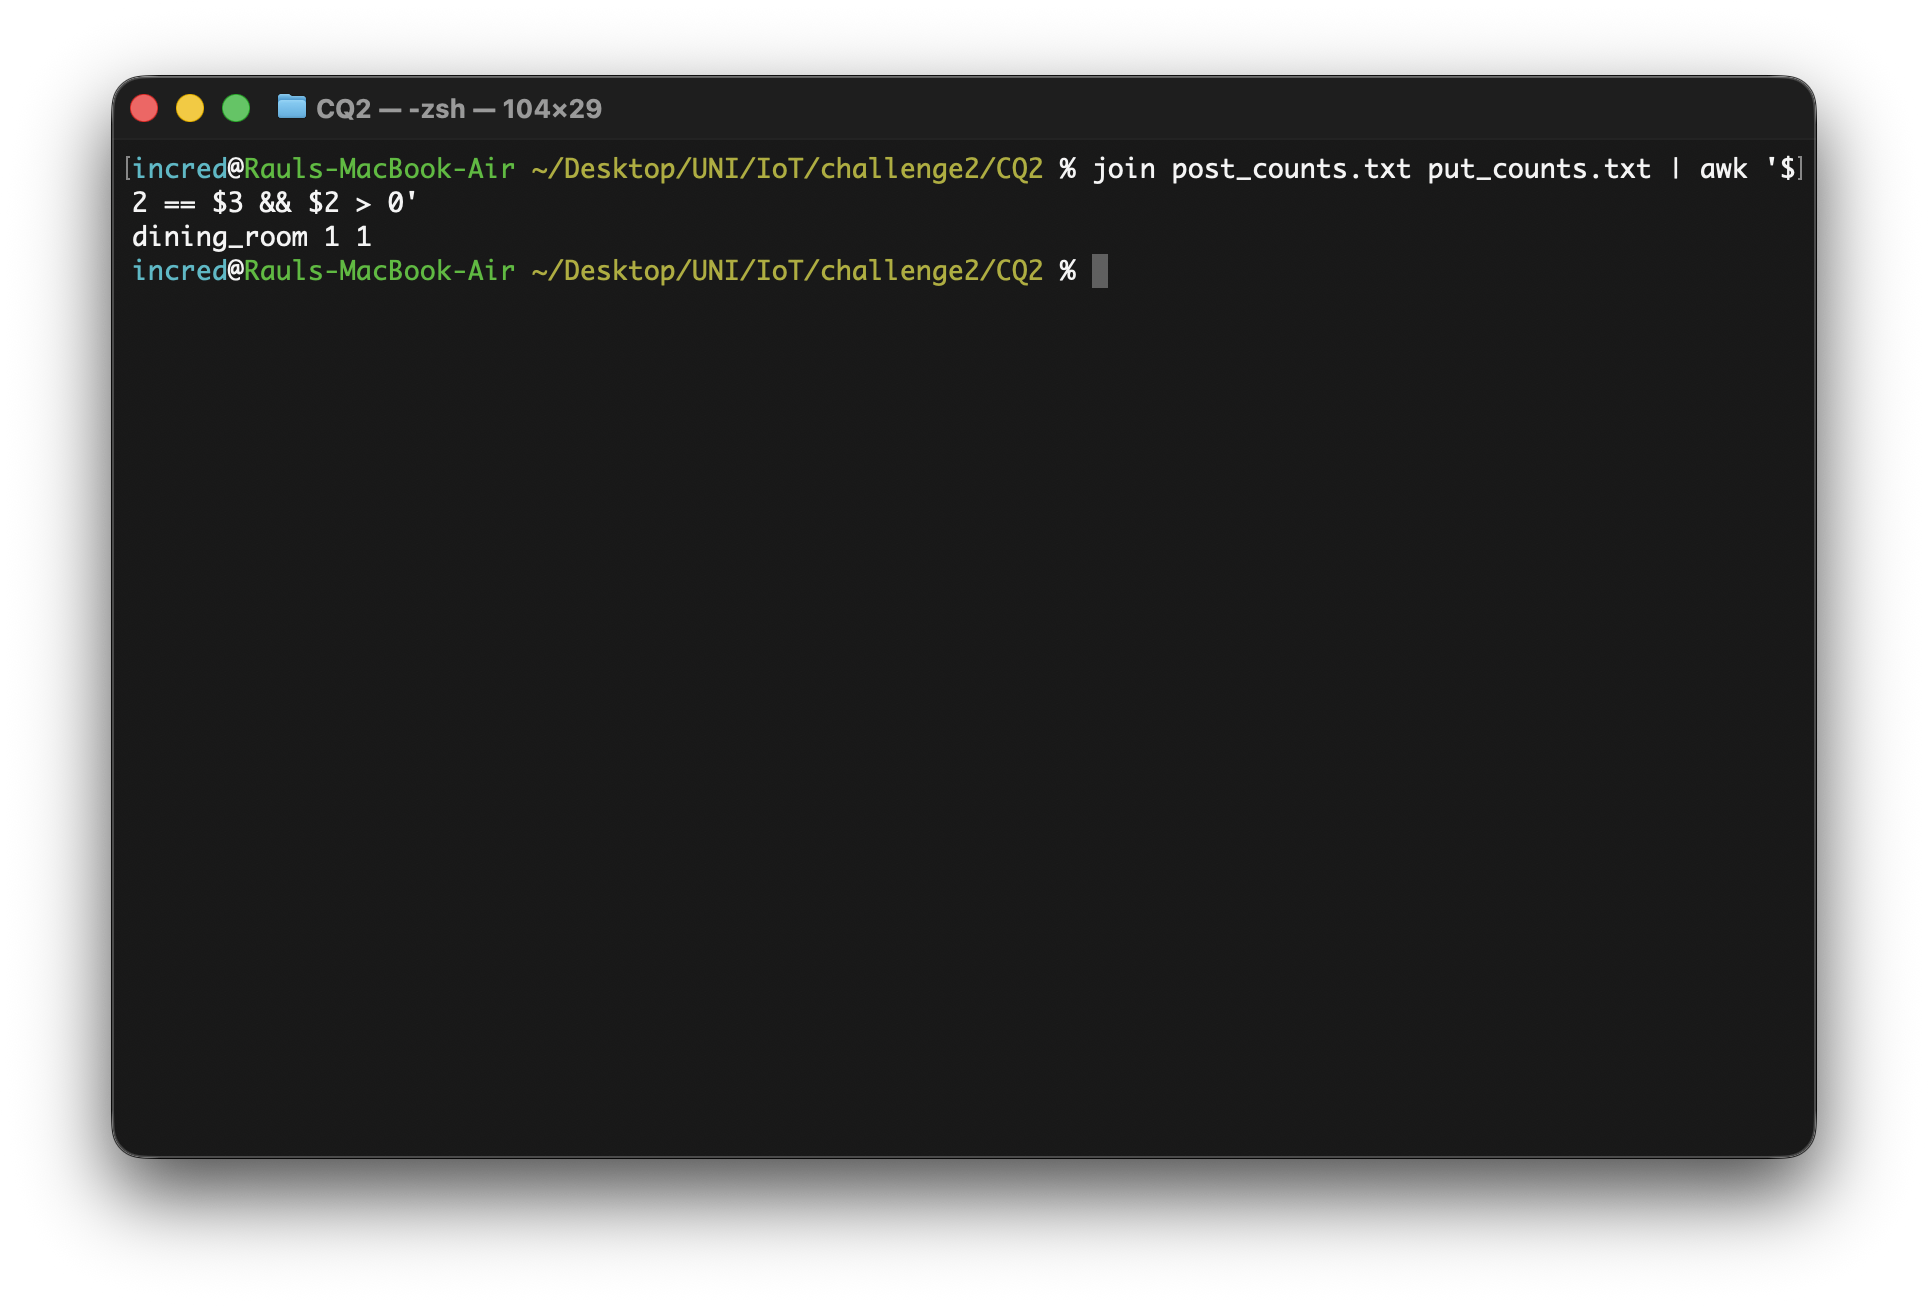
\includegraphics[width=0.75\linewidth]{images/cq2-result.png}
\end{figure}

\vspace{0.3cm}

\textbf{\huge Answer CQ2: 1}
\end{minipage}


\section{CQ3}

\begin{fancyquote}
    \textbf{CQ3a)} How many separate observe notifications have been sent containing values for the resource ``/dining\_room/temperature'', ignoring retransmissions?\\
    \textbf{CQ3b)} How many of the notifications found in point CQ3a) are useless (e.g., a waste of traffic)?
\end{fancyquote}

\vspace{0.3cm}

\noindent
\begin{minipage}{\linewidth}
\subsection*{CQ3a - Identify the Token for \texttt{/dining\_room/temperature}}
Filter the URI path to \texttt{dining\_room/temperature}:
\begin{lstlisting}
tshark -r A.pcapng -Y "coap.code == 1 && coap.opt.observe == 0" -T fields -e coap.token -e coap.opt.uri_path | grep "dining_room,temperature" | awk '{print $1}' | sort -u
\end{lstlisting}
\vspace{-0.2cm}
\begin{figure}[H]
    \centering
    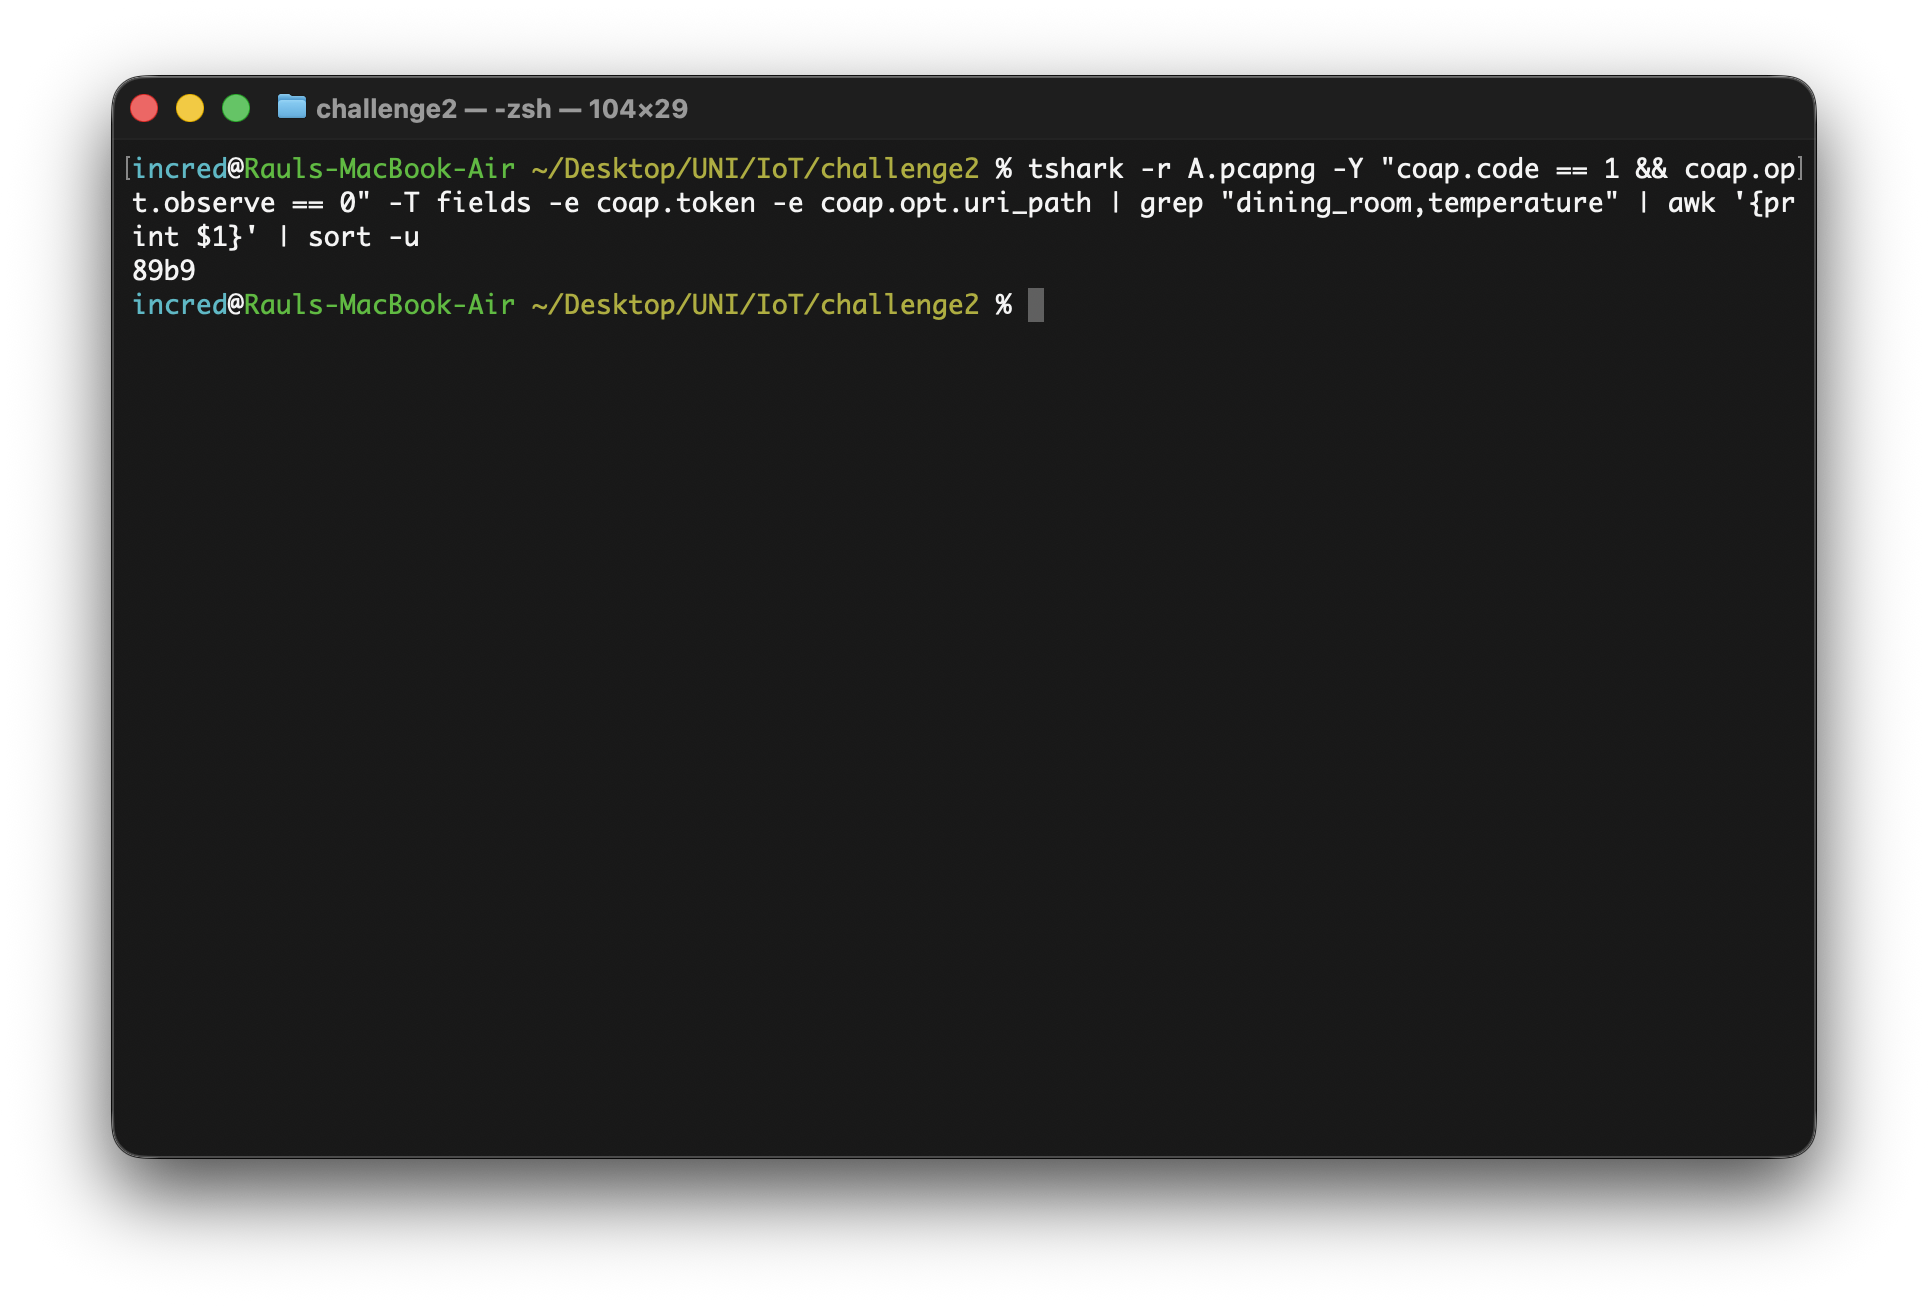
\includegraphics[width=0.75\linewidth]{images/cq3-token.png}
\end{figure}
\end{minipage}

\vspace{0.5cm}

\subsection*{CQ3a - Count Separate Observe Notifications}
Extract the notifications sent by the server. Notifications use the response code \texttt{2.05 Content} (Integer value: 69) and contain the \texttt{coap.opt.observe} field (which acts as a sequence number). To ignore retransmissions, we must filter out packets that have the same Observe sequence number. Retransmitted notifications carry the exact same sequence number as the original.

\vspace{0.2cm}

\noindent
\begin{minipage}{\linewidth}
\subsubsection*{Extract all notifications for the token}
\begin{lstlisting}
tshark -r A.pcapng -Y "coap.code == 69 && coap.opt.observe" -T fields -e coap.token -e coap.opt.observe -e coap.payload | grep -f CQ3/obs_token.txt > CQ3/all_notifications.txt
\end{lstlisting}
Extracts the Token, Observe Sequence Number, and Payload for all notifications, filtering strictly for the Token.
\vspace{0.1cm}
\begin{figure}[H]
    \centering
    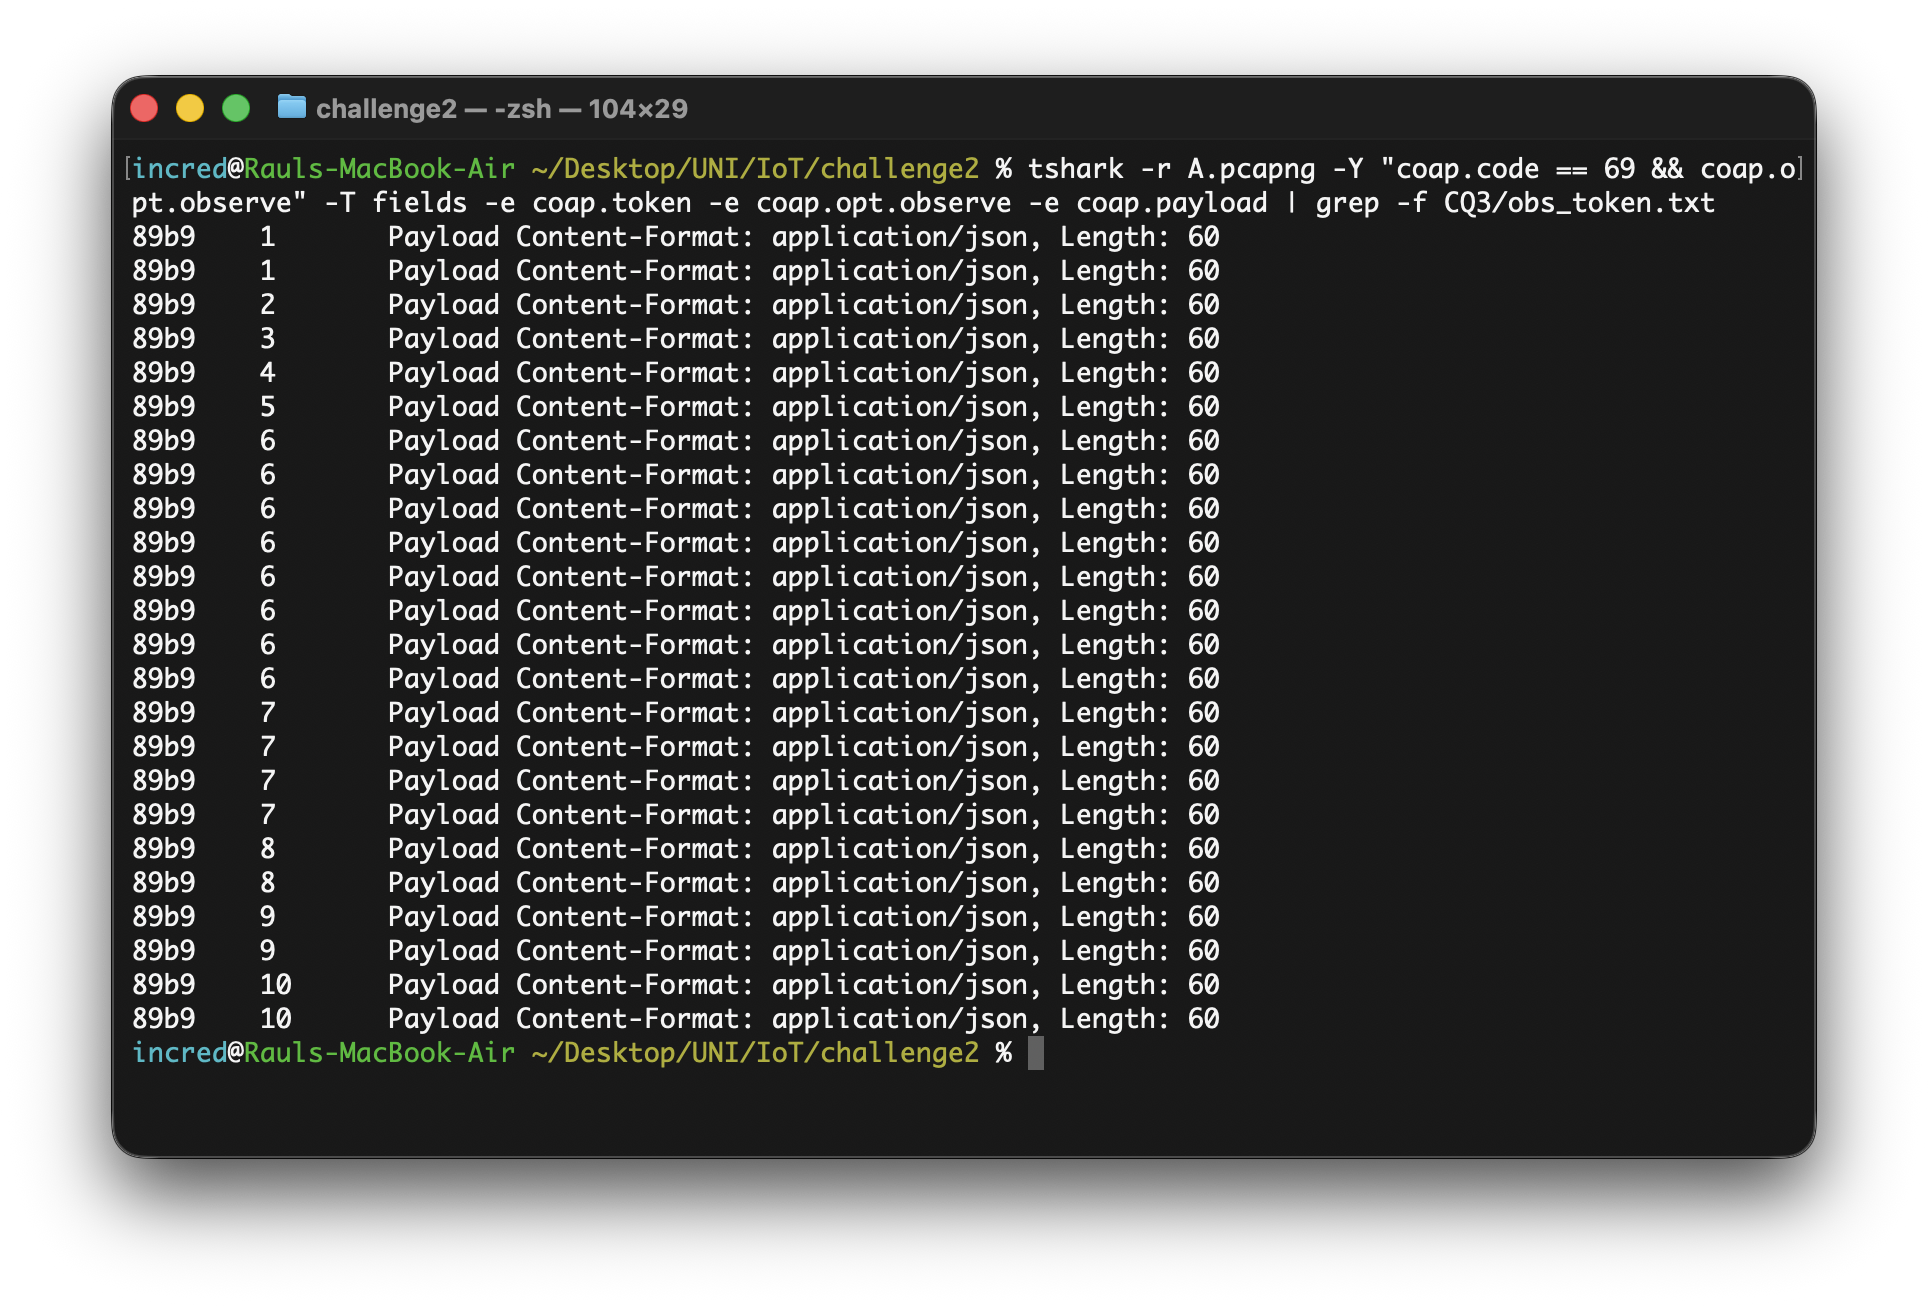
\includegraphics[width=0.75\linewidth]{images/cq3-notifications.png}
\end{figure}
\end{minipage}

\vspace{0.5cm}

\noindent
\begin{minipage}{\linewidth}
\subsubsection*{Filter retransmissions and count}
\begin{lstlisting}
sort -u -k2,2n CQ3/all_notifications.txt > CQ3/unique_notifications.txt
wc -l < CQ3/unique_notifications.txt
\end{lstlisting}
\textbf{\texttt{sort -u -k2,2n}}: Sorts the file numerically (\texttt{n}) based purely on the second column (\texttt{-k2,2}), which is the Observe Sequence Number. The \texttt{-u} flag ensures that if multiple packets have the exact same sequence number (retransmissions), only the first one is kept.
\vspace{0.1cm}
\begin{figure}[H]
    \centering
    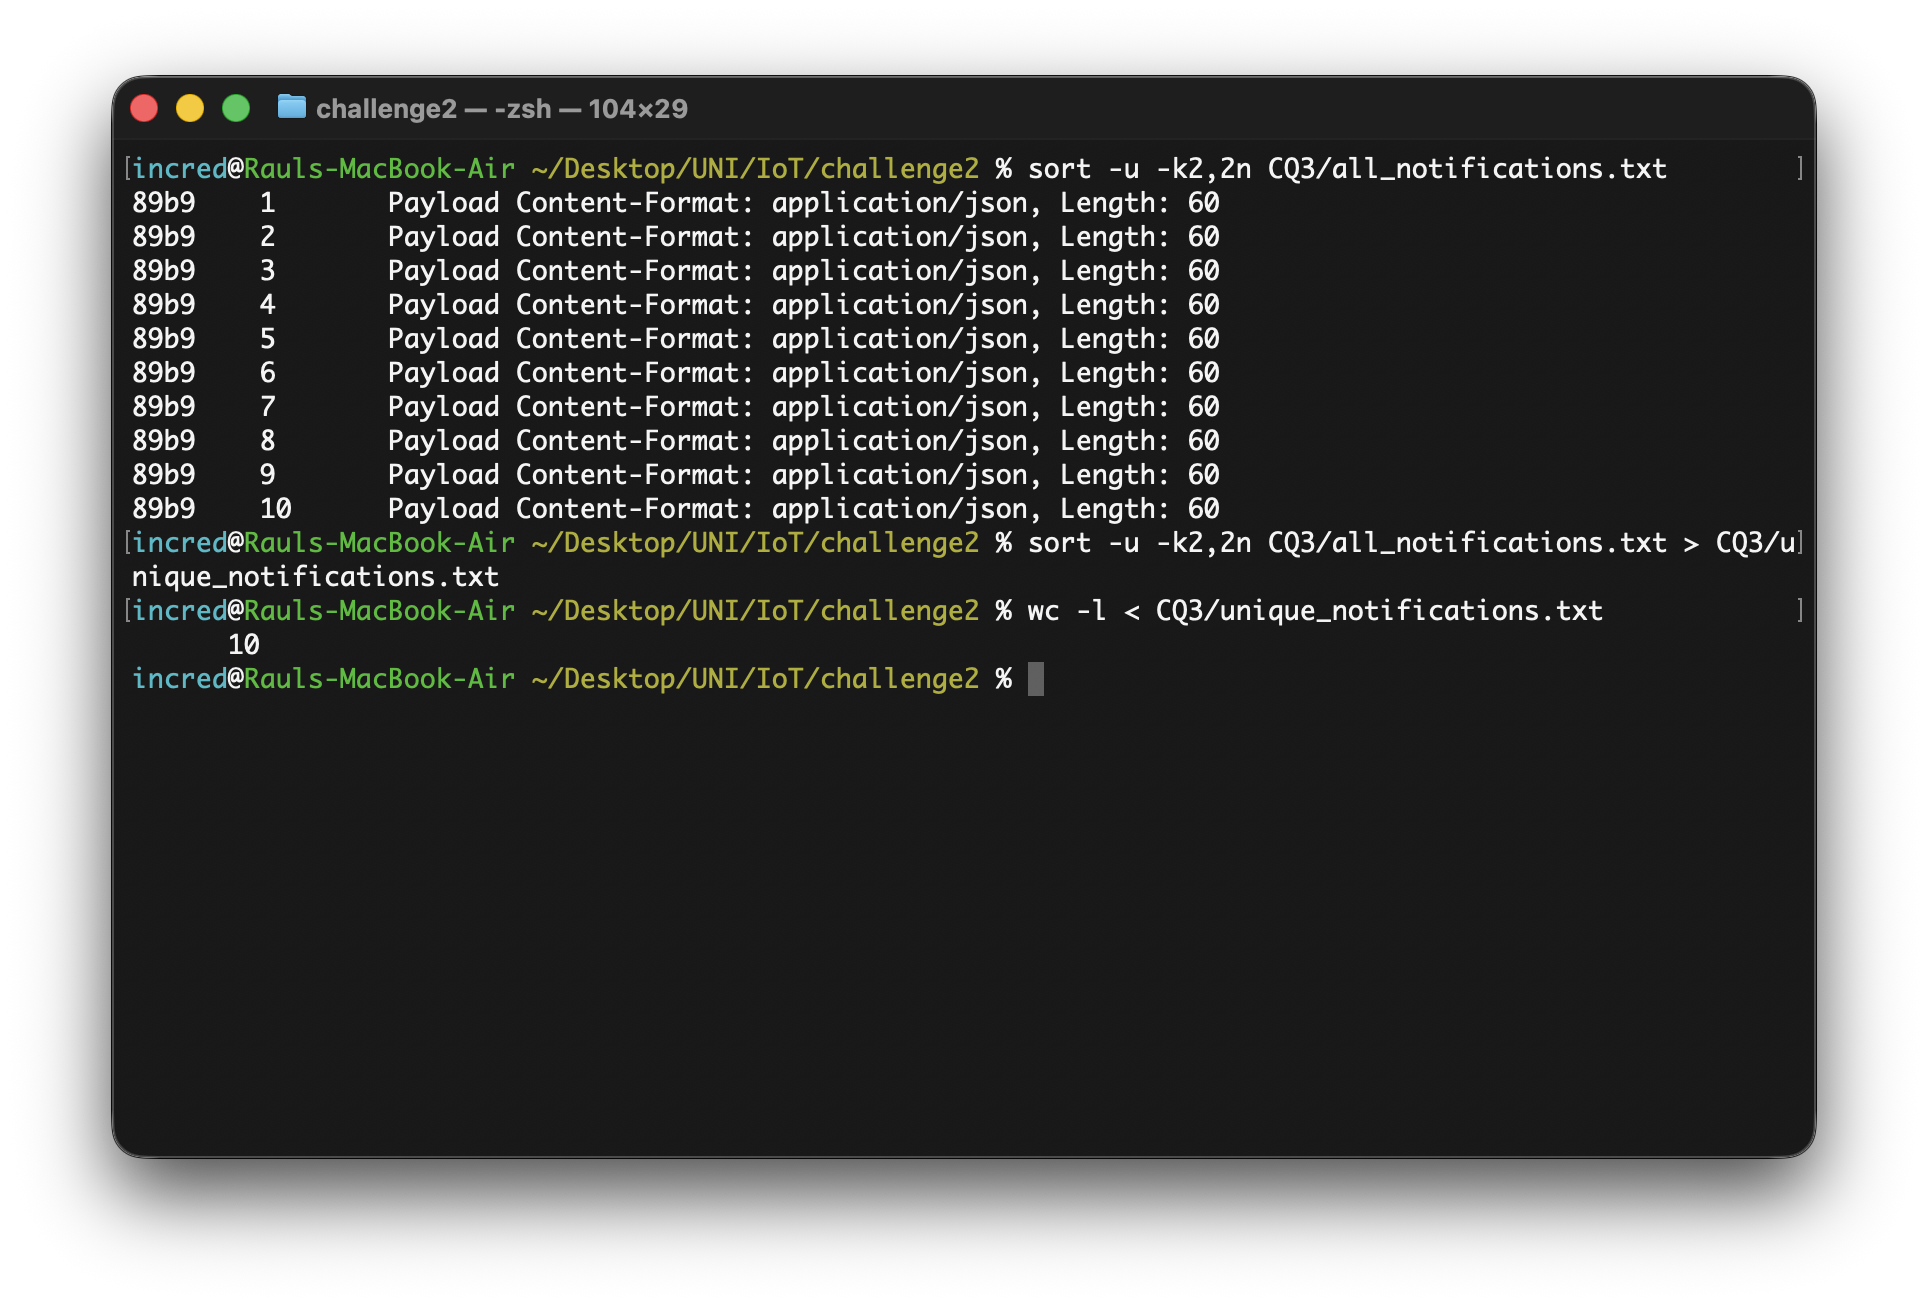
\includegraphics[width=0.75\linewidth]{images/cq3a-result.png}
\end{figure}

\vspace{0.2cm}
\textbf{\huge Answer CQ3a: 10}
\end{minipage}

\noindent
\begin{minipage}{\linewidth}
\subsection*{CQ3b - How many notifications are useless?}

For CQ3b, only the notifications already identified in CQ3a must be considered, therefore retransmissions remain excluded.  
Based on the clarification given for the assignment, a notification should be considered mainly useless if it is sent but not effectively received/processed.

First, I listed the 10 unique notifications found in CQ3a together with their CoAP type, MID, and Observe sequence number:

\begin{lstlisting}
tshark -r A.pcapng -Y "coap.token == 89b9 && coap.code == 69 && coap.opt.observe" -T fields -e frame.number -e coap.type -e coap.mid -e coap.opt.observe | sort -u -k4,4n
\end{lstlisting}

This produced:

\begin{verbatim}
4344  2  10588  1
5098  0  38     2
5623  0  43     3
8509  0  45     4
9414  0  49     5
9866  0  54     6
10573 0  62     7
11220 0  74     8
11917 0  87     9
12782 0  90     10
\end{verbatim}

The first notification is already an ACK-type message (\texttt{coap.type == 2}), while the others are Confirmable notifications (\texttt{coap.type == 0}).  
For each Confirmable notification, I checked whether a corresponding ACK with the same MID exists:

\begin{lstlisting}
tshark -r A.pcapng -Y "coap.type == 2 && (coap.mid == 38 || coap.mid == 43 || coap.mid == 45 || coap.mid == 49 || coap.mid == 54 || coap.mid == 62 || coap.mid == 74 || coap.mid == 87 || coap.mid == 90)" -T fields -e frame.number -e coap.mid
\end{lstlisting}

The result was:

\begin{verbatim}
5099  38
5629  43
8510  45
9415  49
\end{verbatim}

Therefore, ACKs were found only for MIDs \texttt{38}, \texttt{43}, \texttt{45}, and \texttt{49}.  
No ACK was found for MIDs:

\begin{verbatim}
54, 62, 74, 87, 90
\end{verbatim}

These 5 notifications were sent but do not appear to have been successfully confirmed, so they are considered useless according to the intended interpretation of the question.

\vspace{0.4cm}
\textbf{\huge Answer CQ3b: 5}
\end{minipage}


\section{CQ4}

\begin{fancyquote}
    \textbf{Question:}\\
    How many MQTT-SN messages are received by the clients from the local broker listening on port 1885?
\end{fancyquote}

\vspace{0.3cm}

\noindent
\begin{minipage}{\linewidth}
Because MQTT-SN operates over UDP, Tshark does not automatically decode traffic on port 1885 as MQTT-SN. To accurately find messages sent \textit{from} the broker \textit{to} the clients, the first logical step is explicitly forcing the analyzer to interpret all UDP traffic on that specific port as MQTT-SN using the \texttt{-d udp.port==1885,mqttsn} flag. 

Next, we apply a display filter (\texttt{udp.srcport == 1885 \&\& mqttsn}). Filtering by the source port isolates traffic originating from the broker, while adding the \texttt{\&\& mqttsn} condition ensures the packet is not just random UDP noise, but a successfully parsed, valid MQTT-SN message. Finally, we pipe the output to \texttt{wc -l} to count the frames.

\begin{lstlisting}
tshark -r A.pcapng -d udp.port==1885,mqttsn -Y "udp.srcport == 1885 && mqttsn" -T fields -e frame.number | wc -l
\end{lstlisting}

\vspace{0.3cm}

\textbf{\huge Answer CQ4: 0}

\vspace{0.2cm}
\textit{Note: The command outputs \texttt{0}. Further analysis of the PCAP file confirms that while clients send telemetry data to port 1885, the broker never sends any outbound replies from that port. Therefore, the clients received exactly 0 messages from the local broker.}
\end{minipage}

\section{CQ5}

\begin{fancyquote}
    \textbf{Question:}\\
    How many MQTT subscribers receive a last will message derived from a subscription that includes at least one wildcard?
\end{fancyquote}

\subsection*{Identify Clients that Generate a Last Will}
A Last Will message is only published by the broker if a client sets the Will Flag in its \texttt{CONNECT} packet and subsequently disconnects without sending a graceful MQTT \texttt{DISCONNECT}. 

First, extract all clients that configured a Last Will topic:

\begin{lstlisting}[language=bash]
tshark -r B.pcapng -Y "mqtt.conflag.willflag == 1" -T fields -e frame.number -e tcp.stream -e mqtt.clientid -e mqtt.willtopic > will_connects.txt
\end{lstlisting}

Next, extract all graceful MQTT \texttt{DISCONNECT} packets:

\begin{lstlisting}[language=bash]
tshark -r B.pcapng -Y "mqtt.msgtype == 14" -T fields -e frame.number -e tcp.stream > disconnects.txt
\end{lstlisting}

By comparing the two lists, we can isolate the Will-configured streams that dropped ungracefully:

\begin{lstlisting}[language=bash]
awk 'NR==FNR {d[$2]=1; next} !($2 in d) {print}' disconnects.txt will_connects.txt > will_without_disconnect.txt
\end{lstlisting}

This produces the following list of candidate Last Will generators and their respective topics:

\begin{verbatim}
4    0    [missing]          university/department12/room1/temperature
196  12   wikdxsrbyewyocm    metaverse/room2/floor4
352  16   lstvfjwz           hospital/facility3/area3
557  21   kiurrznrgj         metaverse/room2/room2
\end{verbatim}

\subsection*{Find Broker-to-Subscriber Deliveries on Will Topics}
To determine which of these messages were actually distributed, we must extract all MQTT \texttt{PUBLISH} packets matching the candidate Will topics:

\begin{lstlisting}[language=bash]
tshark -r B.pcapng -Y 'mqtt.msgtype == 3 && (mqtt.topic == "hospital/facility3/area3" || mqtt.topic == "metaverse/room2/floor4" || mqtt.topic == "metaverse/room2/room2" || mqtt.topic == "university/department12/room1/temperature")' -T fields -e frame.number -e tcp.stream -e ip.src -e ip.dst -e tcp.srcport -e tcp.dstport -e mqtt.topic > will_publishes.txt
\end{lstlisting}

To filter exclusively for messages delivered \emph{by the broker} to the subscribers, we isolate packets originating from the default MQTT source port (\texttt{1883}):

\begin{lstlisting}[language=bash]
awk -F '\t' '$5 == "1883" {print}' will_publishes.txt > will_delivered.txt
\end{lstlisting}

We then associate each delivery stream with its corresponding MQTT client identifier to map the exact recipients:

\begin{lstlisting}[language=bash]
tshark -r B.pcapng -Y "mqtt.msgtype == 1" -T fields -e tcp.stream -e mqtt.clientid | sort -u > stream_clientid.txt
awk 'NR==FNR {cid[$1]=$2; next} {print $1, $2, cid[$2]}' stream_clientid.txt will_delivered.txt > actual_will_delivered_with_client.txt
\end{lstlisting}


\subsection*{Intersect Deliveries with Wildcard Subscriptions}
The objective requires identifying subscribers that receive the Last Will \emph{specifically due to a wildcard subscription}. First, extract all \texttt{SUBSCRIBE} requests containing wildcards (\texttt{+} or \texttt{\#}) and map them to their client identifiers:

\begin{lstlisting}[language=bash]
tshark -r B.pcapng -Y "mqtt.msgtype == 8" -T fields -e frame.number -e tcp.stream -e mqtt.topic | grep -E '\+|#' > wildcard_subs.txt
awk 'NR==FNR {cid[$1]=$2; next} {print $1, $2, cid[$2], $3}' stream_clientid.txt wildcard_subs.txt > wildcard_subs_with_client.txt
\end{lstlisting}

Reviewing the valid deliveries reveals that the only relevant active Will topic is:
\begin{verbatim}
university/department12/room1/temperature
\end{verbatim}

The active wildcard subscriptions capable of matching this specific topic are:
\begin{itemize}
    \item \texttt{university/\#}
    \item \texttt{university/+/+/\#}
\end{itemize}

Finally, we compute the intersection between clients holding these specific wildcard subscriptions and the clients that actually received the Will message:

\begin{lstlisting}[language=bash]
awk '$4=="university/#" || $4=="university/+/+/#"' wildcard_subs_with_client.txt | awk '{print $3}' | sort -u > cq5_wild_subscribers.txt
awk '$3!="" {print $3}' actual_will_delivered_with_client.txt | sort -u > cq5_will_receivers.txt
comm -12 cq5_wild_subscribers.txt cq5_will_receivers.txt
\end{lstlisting}

This intersection returns a single client ID: \texttt{zmjnxudohrkaegmh}. \\

\vspace{0.5cm}
\noindent
\textbf{\huge Answer CQ5: 1} \\
(Only one MQTT subscriber receives a Last Will message derived from a wildcard subscription).

\section{CQ6}

\begin{fancyquote}
    \textbf{CQ6a)} How many different MQTT clients sent atleast one message to erase a previously retained value in a topic in the public HiveMQ broker?\\
    \textbf{CQ6b)} How many of the clients found in CQ6a) connected to the HiveMQ broker with a client identifier strictly longer than 7 bytes (>7)?
\end{fancyquote}

To solve the question, we first identified the IP addresses of the public HiveMQ broker from DNS resolution:
\begin{lstlisting}
tshark -r B.pcapng -Y 'dns.flags.response == 1 && dns.qry.name contains "hivemq"' -T fields -e dns.qry.name -e dns.a
\end{lstlisting}
\[
35.158.43.69,\; 35.158.34.213,\; 18.192.151.104
\]

Then we considered only MQTT traffic directed to those IP addresses.

In MQTT, a retained value is erased by sending a \texttt{PUBLISH} message with:
\begin{itemize}
    \item \texttt{mqtt.msgtype == 3} (\texttt{PUBLISH})
    \item retain flag set
    \item empty payload
\end{itemize}

Therefore, the solution was structured in two parts:
\begin{enumerate}
    \item map each TCP stream to the corresponding MQTT client identifier using \texttt{CONNECT} packets;
    \item find the TCP streams containing retained \texttt{PUBLISH} messages with empty payload, then associate those streams with their client identifiers.
\end{enumerate}

\subsection*{1. Extract MQTT client identifiers from CONNECT packets}

We extracted all MQTT \texttt{CONNECT} packets directed to the HiveMQ broker and saved the mapping \texttt{tcp.stream $\rightarrow$ mqtt.clientid}:

\begin{lstlisting}
tshark -r B.pcapng -Y '(ip.dst == 35.158.43.69 || ip.dst == 35.158.34.213 || ip.dst == 18.192.151.104) && mqtt.msgtype == 1' -T fields -e tcp.stream -e mqtt.clientid | sort -u > stream_clientid.txt
\end{lstlisting}

This produced the following stream-to-client mapping:

    \begin{verbatim}
    1   pcbtjyj
    3   cpoepjzkhibxgjiu
    8   dzcxnwdqef
    15  tukvxesuhe
    20  fcthvjikxjul
    22  giuxfijwus
    23  pohujuv
    43  atqeblw
    44  rolsmcwhshlbc
    \end{verbatim}


\subsection*{2. Find retained PUBLISH messages with empty payload}

Then we extracted all retained MQTT \texttt{PUBLISH} packets directed to the HiveMQ broker:

\begin{lstlisting}
tshark -r B.pcapng -Y "($BROKER_DST) && mqtt.msgtype == 3 && mqtt.retain == 1" -T fields -e frame.number -e tcp.stream -e mqtt.topic -e mqtt.msg -e mqtt.msg_text > retained_candidates.txt
\end{lstlisting}

In the output, packets used to erase a retained value are those where the payload field is missing, shown by \texttt{<MISSING>}.  
Thus we extracted the corresponding TCP streams:

\begin{lstlisting}
awk -F '\t' '($4 == "<MISSING>" || $4 == "") {print $2}' retained_candidates.txt | sort -u > erase_streams.txt
\end{lstlisting}
The resulting streams were:
    \begin{verbatim}
    1
    22
    23
    43
    44
    \end{verbatim}

\subsection*{3. Associate erase streams with client identifiers}

Finally, we associated the streams found above with the client identifiers extracted from the \texttt{CONNECT} packets:

\begin{lstlisting}
sort erase_streams.txt > erase_streams_sorted.txt
sort stream_clientid.txt > stream_clientid_sorted.txt
join erase_streams_sorted.txt stream_clientid_sorted.txt > cq6_clients.txt
\end{lstlisting}

So the distinct MQTT clients that sent at least one retained-delete message are:
\[
\{\texttt{pcbtjyj},\; \texttt{giuxfijwus},\; \texttt{pohujuv},\; \texttt{atqeblw},\; \texttt{rolsmcwhshlbc}\}
\]

\textbf{\huge Answer CQ6a: 5}

\subsection*{4. Count client identifiers longer than 7 bytes}

Among the 5 clients found in CQ6a:
\begin{itemize}
    \item \texttt{pcbtjyj} has length 7
    \item \texttt{giuxfijwus} has length 10
    \item \texttt{pohujuv} has length 7
    \item \texttt{atqeblw} has length 7
    \item \texttt{rolsmcwhshlbc} has length 13
\end{itemize}

Therefore, the client identifiers strictly longer than 7 bytes are:
\[
\texttt{giuxfijwus},\; \texttt{rolsmcwhshlbc}
\]

\textbf{\huge Answer CQ6b: 2}
\section{CQ7}

\begin{fancyquote}
    \textbf{Question:}\\
    How many MQTT subscribe requests directed to the local broker specify a topic with at least two wildcards?
\end{fancyquote}

We extracted all MQTT \texttt{SUBSCRIBE} packets from \texttt{B.pcapng}:

\begin{lstlisting}
tshark -r B.pcapng -Y "mqtt.msgtype == 8" -T fields -e frame.number -e tcp.stream -e ip.src -e ip.dst -e mqtt.topic > all_subscribe.txt
\end{lstlisting}

Then we filtered the subscribe requests whose topic filter contains at least two wildcard symbols.  
In MQTT, the wildcard symbols are:
\begin{itemize}
    \item \texttt{+} for single-level wildcard
    \item \texttt{\#} for multi-level wildcard
\end{itemize}

To detect topics containing at least two wildcards, we used:

\begin{lstlisting}
awk -F '\t' '$5 ~ /[+#].*[+#]/ {print $0}' all_subscribe.txt
\end{lstlisting}

This produced the following candidate subscribe requests:

\begin{verbatim}
226   university/+/+/deposit
363   hospital/+/+/light
375   university/+/+/#
460   metaverse/+/room1/#
473   house/department3/+/+
700   metaverse/facility0/+/+
1177  hospital/fxlugs/+/#
1915  metaverse/+/+/hydraulic_valve
2360  factory/+/#
2994  house/+/room1/#
\end{verbatim}

However, the request in frame \texttt{375} was directed to \texttt{18.192.151.104}, which is a public HiveMQ broker and not the local broker. Therefore, it must be excluded.

The remaining valid subscribe requests directed to the local broker are:

\begin{verbatim}
226   university/+/+/deposit
363   hospital/+/+/light
460   metaverse/+/room1/#
473   house/department3/+/+
700   metaverse/facility0/+/+
1177  hospital/fxlugs/+/#
1915  metaverse/+/+/hydraulic_valve
2360  factory/+/#
2994  house/+/room1/#
\end{verbatim}

Therefore, the total number of MQTT subscribe requests directed to the local broker that specify a topic with at least two wildcards is:\\

\textbf{\huge Answer CQ7: 9}
\section{CQ8}

\begin{fancyquote}
    \textbf{Question:}\\
    Compare the local broker usage in the two capture files \texttt{A.pcapng} and \texttt{B.pcapng}. The goal is to have a plot on the number of layers of the topics used in the publish messages directed to the local broker in the two captures.
\end{fancyquote}

For this question, we considered only MQTT \texttt{PUBLISH} messages \textbf{directed to the local broker}, i.e.\ messages entering the broker, and not messages sent by the broker to subscribers.

\subsection*{Dataset A}

First, we identified the local broker in \texttt{A.pcapng} by inspecting MQTT \texttt{CONNECT} packets. The relevant connections were directed to \texttt{127.0.0.1:1883}, so the local broker is the loopback broker.

To extract only MQTT \texttt{PUBLISH} packets entering the local broker, we used:

\begin{lstlisting}
tshark -r A.pcapng -Y "mqtt.msgtype == 3 && tcp.dstport == 1883 && ip.dst == 127.0.0.1" -T fields -e frame.number -e tcp.stream -e tcp.srcport -e tcp.dstport -e mqtt.topic > A_publish_into_broker_port1883.txt
\end{lstlisting}

The total number of considered publish messages is obtained with:

\begin{lstlisting}
wc -l < A_publish_into_broker_port1883.txt
\end{lstlisting}

which gives:

\begin{verbatim}
439
\end{verbatim}

Then we computed the number of topic layers by splitting each topic on the \texttt{/} character:

\begin{lstlisting}
awk -F '\t' '{
    topic=$5;
    n=split(topic,a,"/");
    print n
}' A_publish_into_broker_port1883.txt | sort -n | uniq -c
\end{lstlisting}

This produced:

\begin{verbatim}
154 2
131 3
154 4
\end{verbatim}

So for \texttt{A.pcapng}:
\begin{itemize}
    \item Layer 1: 0
    \item Layer 2: 154
    \item Layer 3: 131
    \item Layer 4: 154
\end{itemize}

\subsection*{Dataset B}

For \texttt{B.pcapng}, we first extracted all MQTT \texttt{PUBLISH} messages directed to brokers on port \texttt{1883}:

\begin{lstlisting}
tshark -r B.pcapng -Y "mqtt.msgtype == 3 && tcp.dstport == 1883" -T fields -e frame.number -e ip.src -e ip.dst -e tcp.srcport -e tcp.dstport -e mqtt.topic > B_publish_to_brokers.txt
\end{lstlisting}

By checking the IPv4 and IPv6 destination fields, we observed that the local broker traffic appears on loopback IPv6 (\texttt{::1}), while the public HiveMQ traffic uses external IPv4 addresses. In the original extraction, these loopback IPv6 packets appeared with an empty \texttt{ip.dst} field. Therefore, we isolated local broker publish traffic with:

\begin{lstlisting}
awk -F '\t' '$3 == "" {print}' B_publish_to_brokers.txt > B_local_publish.txt
\end{lstlisting}

The total number of considered publish messages is:

\begin{lstlisting}
wc -l < B_local_publish.txt
\end{lstlisting}

which gives:

\begin{verbatim}
534
\end{verbatim}

Then we computed the number of topic layers with:

\begin{lstlisting}
awk -F '\t' '{
    topic=$6;
    n=split(topic,a,"/");
    print n
}' B_local_publish.txt | sort -n | uniq -c
\end{lstlisting}

This produced:

\begin{verbatim}
21  1
172 2
162 3
179 4
\end{verbatim}

So for \texttt{B.pcapng}:
\begin{itemize}
    \item Layer 1: 21
    \item Layer 2: 172
    \item Layer 3: 162
    \item Layer 4: 179
\end{itemize}

\subsection*{Final result}

The final topic-layer distributions are:

\begin{center}
\begin{tabular}{c|cc}
\textbf{Number of layers} & \textbf{Dataset A} & \textbf{Dataset B} \\
\hline
1 & 0   & 21  \\
2 & 154 & 172 \\
3 & 131 & 162 \\
4 & 154 & 179 \\
\end{tabular}
\end{center}

\begin{figure}[H]
    \centering
    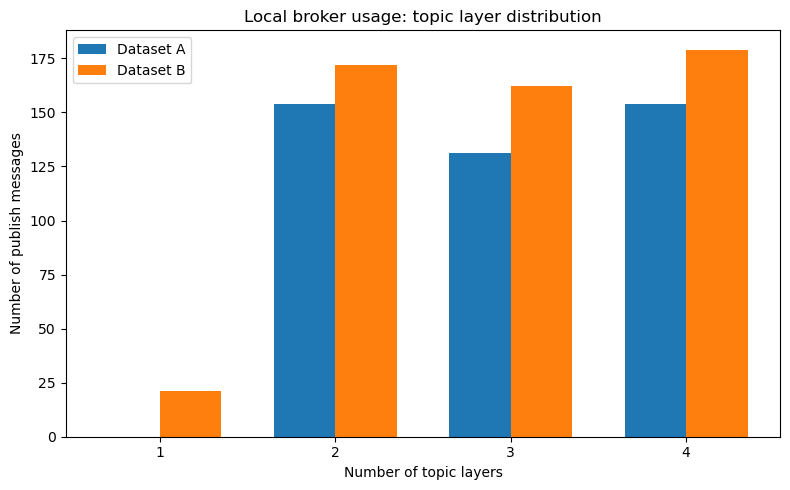
\includegraphics[width=0.75\linewidth]{images/cq8_plot.png}
    \caption{Histogram of the number of topic layers in MQTT \texttt{PUBLISH} messages directed to the local broker, comparing \texttt{A.pcapng} and \texttt{B.pcapng}.}
\end{figure}

The total number of publish messages considered for the analysis is:

\begin{itemize}
    \item \texttt{A.pcapng}: 439
    \item \texttt{B.pcapng}: 534
\end{itemize}

Therefore:

\vspace{0.3cm}

\noindent{\huge\bfseries Answer CQ8a: 439\par}

\vspace{0.3cm}

\noindent{\huge\bfseries Answer CQ8b: 534\par}
% \section{CQ5}

\begin{fancyquote}
    \textbf{Question:}\\
    How many MQTT subscribers receive a last will message derived from a subscription that includes at least one wildcard?
\end{fancyquote}

\subsection*{Identify Clients that Generate a Last Will}
A Last Will message is only published by the broker if a client sets the Will Flag in its \texttt{CONNECT} packet and subsequently disconnects without sending a graceful MQTT \texttt{DISCONNECT}. 

First, extract all clients that configured a Last Will topic:

\begin{lstlisting}[language=bash]
tshark -r B.pcapng -Y "mqtt.conflag.willflag == 1" -T fields -e frame.number -e tcp.stream -e mqtt.clientid -e mqtt.willtopic > will_connects.txt
\end{lstlisting}

Next, extract all graceful MQTT \texttt{DISCONNECT} packets:

\begin{lstlisting}[language=bash]
tshark -r B.pcapng -Y "mqtt.msgtype == 14" -T fields -e frame.number -e tcp.stream > disconnects.txt
\end{lstlisting}

By comparing the two lists, we can isolate the Will-configured streams that dropped ungracefully:

\begin{lstlisting}[language=bash]
awk 'NR==FNR {d[$2]=1; next} !($2 in d) {print}' disconnects.txt will_connects.txt > will_without_disconnect.txt
\end{lstlisting}

This produces the following list of candidate Last Will generators and their respective topics:

\begin{verbatim}
4    0    [missing]          university/department12/room1/temperature
196  12   wikdxsrbyewyocm    metaverse/room2/floor4
352  16   lstvfjwz           hospital/facility3/area3
557  21   kiurrznrgj         metaverse/room2/room2
\end{verbatim}

\subsection*{Find Broker-to-Subscriber Deliveries on Will Topics}
To determine which of these messages were actually distributed, we must extract all MQTT \texttt{PUBLISH} packets matching the candidate Will topics:

\begin{lstlisting}[language=bash]
tshark -r B.pcapng -Y 'mqtt.msgtype == 3 && (mqtt.topic == "hospital/facility3/area3" || mqtt.topic == "metaverse/room2/floor4" || mqtt.topic == "metaverse/room2/room2" || mqtt.topic == "university/department12/room1/temperature")' -T fields -e frame.number -e tcp.stream -e ip.src -e ip.dst -e tcp.srcport -e tcp.dstport -e mqtt.topic > will_publishes.txt
\end{lstlisting}

To filter exclusively for messages delivered \emph{by the broker} to the subscribers, we isolate packets originating from the default MQTT source port (\texttt{1883}):

\begin{lstlisting}[language=bash]
awk -F '\t' '$5 == "1883" {print}' will_publishes.txt > will_delivered.txt
\end{lstlisting}

We then associate each delivery stream with its corresponding MQTT client identifier to map the exact recipients:

\begin{lstlisting}[language=bash]
tshark -r B.pcapng -Y "mqtt.msgtype == 1" -T fields -e tcp.stream -e mqtt.clientid | sort -u > stream_clientid.txt
awk 'NR==FNR {cid[$1]=$2; next} {print $1, $2, cid[$2]}' stream_clientid.txt will_delivered.txt > actual_will_delivered_with_client.txt
\end{lstlisting}


\subsection*{Intersect Deliveries with Wildcard Subscriptions}
The objective requires identifying subscribers that receive the Last Will \emph{specifically due to a wildcard subscription}. First, extract all \texttt{SUBSCRIBE} requests containing wildcards (\texttt{+} or \texttt{\#}) and map them to their client identifiers:

\begin{lstlisting}[language=bash]
tshark -r B.pcapng -Y "mqtt.msgtype == 8" -T fields -e frame.number -e tcp.stream -e mqtt.topic | grep -E '\+|#' > wildcard_subs.txt
awk 'NR==FNR {cid[$1]=$2; next} {print $1, $2, cid[$2], $3}' stream_clientid.txt wildcard_subs.txt > wildcard_subs_with_client.txt
\end{lstlisting}

Reviewing the valid deliveries reveals that the only relevant active Will topic is:
\begin{verbatim}
university/department12/room1/temperature
\end{verbatim}

The active wildcard subscriptions capable of matching this specific topic are:
\begin{itemize}
    \item \texttt{university/\#}
    \item \texttt{university/+/+/\#}
\end{itemize}

Finally, we compute the intersection between clients holding these specific wildcard subscriptions and the clients that actually received the Will message:

\begin{lstlisting}[language=bash]
awk '$4=="university/#" || $4=="university/+/+/#"' wildcard_subs_with_client.txt | awk '{print $3}' | sort -u > cq5_wild_subscribers.txt
awk '$3!="" {print $3}' actual_will_delivered_with_client.txt | sort -u > cq5_will_receivers.txt
comm -12 cq5_wild_subscribers.txt cq5_will_receivers.txt
\end{lstlisting}

This intersection returns a single client ID: \texttt{zmjnxudohrkaegmh}. \\

\vspace{0.5cm}
\noindent
\textbf{\huge Answer CQ5: 1} \\
(Only one MQTT subscriber receives a Last Will message derived from a wildcard subscription).
\end{document}
